% science_template.tex
% See accompanying readme.txt for copyright statement, change log etc.

% Any modification of this template, including writing a paper using it,
% MUST rename the file i.e. use a different file name.

%%%%%%%%%%%%%%%% START OF PREAMBLE %%%%%%%%%%%%%%%

% Basic setup. Authors shouldn't need to adjust these commands.
% It's annoying, but please do NOT strip these into a separate file.
% They need to be included in this .tex for our production software to work.

% Use the basic LaTeX article class, 12pt text
\documentclass[12pt]{article}

% Science uses Times font. If you don't have this installed (most LaTeX installations will be
% fine) or prefer the old Computer Modern fonts, comment out the following line
\usepackage{newtxtext,newtxmath}
% Depending on your LaTeX fonts installation, you might get better results with one or both of these:
%\usepackage{mathptmx}
%\usepackage{txfonts}

\usepackage[right]{lineno}

% Allow external graphics files
\usepackage{graphicx}

% Use US letter sized paper with 1 inch margins
\usepackage[letterpaper,margin=1in]{geometry}

% Double line spacing, including in captions
\linespread{1.5} % For some reason double spacing is 1.5, not 2.0!

% One space after each sentence
\frenchspacing

% Abstract formatting and spacing - no heading
\renewenvironment{abstract}
    {\quotation}
    {\endquotation}

% No date in the title section
\date{}

% Reference section heading
\renewcommand\refname{References and Notes}

% Figure and Table labels in bold
\makeatletter
\renewcommand{\fnum@figure}{\textbf{Figure \thefigure}}
\renewcommand{\fnum@table}{\textbf{Table \thetable}}
\makeatother

% Call the accompanying scicite.sty package.
% This formats citation numbers in Science style.
\usepackage{scicite}

% Provides the \url command, and fixes a crash if URLs or DOIs contain underscores
\usepackage{url}

%%%%%%%%%%%% CUSTOM COMMANDS AND PACKAGES %%%%%%%%%%%%

% Authors can define simple custom commands e.g. as shortcuts to save on typing
% Use \newcommand (not \def) to avoid overwriting existing commands.
% Keep them as simple as possible and note the warning in the text below.
% Example:
\newcommand{\pcc}{\,cm$^{-3}$}  % per cm-cubed

% Please DO NOT import additional external packages or .sty files.
% Those are unlikely to work with our conversion software and will cause problems later.
% Don't add any more \usepackage{} commands.


%%%%%%%%%%%%%%%% TITLE AND AUTHORS %%%%%%%%%%%%%%%%

\def\scititle{
    A geographic history of human genetic ancestry
}
% Store the title in a variable for reuse in the supplement (otherwise \maketitle deletes it)
\title{\bfseries \boldmath \scititle}

% Author and institution list.
% Institution numbers etc. should be hard-coded, do *not* use the \footnote command.
\author{
    % You can write out first names or use initials - either way is acceptable, but be consistent
    Michael~C.~Grundler$^{1}$,
    Jonathan~Terhorst$^{2}$,
    Gideon~S.~Bradburd$^{1\ast}$\and
    % Additional lines of authors should be inserted using the \and command (not \\)
    % Institution list, in a slightly smaller font
    \small$^{1}$Department of Ecology and Evolutionary Biology, University of Michigan, Ann Arbor, MI 48109, USA.\and
    \small$^{2}$Department of Statistics, University of Michigan, Ann Arbor, MI 48109, USA.\and
    % Identify at least one corresponding author, with contact email address
    \small$^\ast$Corresponding author. Email: bradburd@umich.edu
}

%%%%%%%%%%%%%%%%% END OF PREAMBLE %%%%%%%%%%%%%%%%

%%%%%%%%%%%%%%%% START OF MAIN TEXT %%%%%%%%%%%%%%%
\begin{document} 

% Insert the title and author list
\maketitle

\begin{linenumbers}

% Abstract, in bold
% There are strict length limits, and not all formats have abstracts.
% Consult the journal instructions to authors for details.
% Do not cite any references in the abstract.
\begin{abstract} \bfseries \boldmath
Describing the distribution of genetic variation across individuals is a
fundamental goal of population genetics. We present a method that capitalizes
on the rich genealogical information encoded in genomic tree sequences to infer
the geographic locations of the shared ancestors of a sample of sequenced
individuals. We use this method to infer the geographic history of genetic
ancestry of a set of human genomes sampled from Europe, Asia, and Africa,
accurately recovering major population movements on those continents. Our
findings demonstrate the importance of defining the spatial-temporal context of
genetic ancestry to describing human genetic variation and caution against the
oversimplified interpretations of genetic data prevalent in contemporary
discussions of race and ancestry.
\end{abstract}


% The first paragraph of any Science paper does NOT have a heading
% Nor is it indented
\noindent Present-day genomes are inherited from an an unbroken chain of
ancestors who lived in different geographic locations at different times,
creating spatial patterns of genetic relatedness~\cite{Bradburd_Ralph_2019}. 
Understanding these spatial patterns is vital both for the identification of
the genomic basis of phenotypic variation~\cite{battey2020} and for knowledge 
of the demographic history of a species~e.g.\cite{Ralph2013}. Conversely,
ignoring spatial demographic history can have serious implications for
genome-wide association studies or the identification of loci involved in local
adaptation~\cite{zaidi2020}.

Genetic variation in humans is often summarized with discrete geographic labels,
but these can be inaccurate and misleading~\cite{Coop_2022, lewis2023}. Even
when loosely based on geographic history, genetic ancestry labels oversimplify
a complex picture because they implicitly focus on only a single point in time.
For example, based on our current best understanding of human origins, all
living individuals are ``African" (regardless of the geography of their recent
ancestors) on considering their ancestry $\sim$200~ky before present. Advances
in the study of ancient DNA have revealed a lack of genetic continuity within
geographic regions e.g.~\cite{Haak2015, allentoft2015population, racimo2020,
mattila2023}, further highlighting the shortcomings of genetic ancestry labels.
The fact that these labels are generated using statistical genetics approaches
gives them the veneer of authenticity, further reifying problematic notions of
race and ancestry in society~\cite{lewis2023, carlson2022}.

At a technical level, many of the existing statistical methods for quantifying
ancestry average over the ages of shared ancestors in the sample, effectively
``flattening" the temporal component of the genealogy that connects all
individuals within a species~\cite{Lawson_etal_2012,Pritchard_etal_2000}. In
reality, any pair of individuals is connected by many shared ancestors from
whom each has inherited some portion of their genome~\cite{Mathieson_Scally_2020}. 
This flattening has the effect of painting a static notion of ancestry, rather 
than one that changes as it proceeds backwards in time.

If we knew the identities, locations, and ages of the ancestors of a sample, we
could much more precisely and accurately report the geographic ancestry of a
set of modern-day individuals through time. Moreover, we could learn about the
history of dispersal in a species, identifying major population movements,
demographic events, and barriers to migration. Although such detailed pedigree
information is rarely available [but see \cite{Aguillon2017} and \cite{anderson2023}], 
it nevertheless is possible to learn about the pedigree ancestors that are shared 
among individuals in a sample. This is because genetic relationships between samples, 
as well as the identities of the shared ancestors via whom they are related, are 
encoded in an interwoven collection of gene genealogies called an ancestral 
recombination graph (ARG)~\cite{griffiths1997,lewanski2024,wong2023ARGs}.

Recent advances in statistical and computational population genetics 
\cite{speidel2019, Kelleher_etal_2019, Wohns_etal_2022, deng2024} have
facilitated the inference of an ARG from large numbers of whole genomes. The
ARG is a record of all coalescence and recombination events since the
divergence of the sequences under study, and therefore specifies a complete
genealogy of the sample at each genomic position. This record can be
represented as a tree sequence \cite{Kelleher_etal_2016, kelleher2018efficient} -- 
an ordered set of trees, localized to adjacent regions of the genome, describing
the gene genealogies of a set of samples at every genomic position. Each
internal node in these local genealogies represents a haplotype within an
ancestor from whom two or more sampled individuals have co-inherited a portion
of their genome. By estimating where and when each of these ancestors lived, we
can, in principle, reconstruct the geographic history of a set of modern day
individuals, documenting the path through space and time by which their genomes
came to them.

Here, we present and validate a method for achieving this goal. Our method,
called \textsc{gaia} (geographic ancestor inference algorithm), efficiently
infers the geographic locations of the shared ancestors of a modern,
georeferenced sample. We apply \textsc{gaia} to a tree sequence of humans
sampled in Europe, Asia, the Middle East, and Africa~\cite{Wohns_etal_2022}, 
and reconstruct the geographic history of human ancestry over the 
last two million years.

\subsection*{Inferring the locations of shared ancestors}

Conceptually, \textsc{gaia} is similar to many tree-based methods in 
phylogeography that attempt to reason about the locations and movements of
genetic ancestors based on the geographic distribution of modern-day samples and
the phylogenetic relationships among them~\cite{Avise_2000, Knowles_Maddison_2002, Knowles_2009}. 
Instead of working with a single gene tree or with a
collection of independent gene trees, however, \textsc{gaia} generates inferences using
a sequence of locally correlated gene trees. In this regard, \textsc{gaia} is
similar to several recent existing methods. For example, \cite{Wohns_etal_2022}
introduced a nonparametric approach that estimates ancestor locations by successively
averaging the coordinates of sample locations in a postorder traversal of a
tree sequence to their most recent common ancestor. In addition, \cite{Osmond_Coop_2021} 
describe a likelihood method for locating genetic ancestors and estimating migration 
rates based on a model of branching Brownian motion utilizing a sample of local 
gene trees from a tree sequence, an approach that was recently extended by
\cite{Deraje_etal_2024} to the full ARG. \textsc{gaia} differs from these
approaches both in its choice of optimality criterion and in its flexible 
representation of geographic space, which can be continuous or discrete.

\textsc{gaia} works by fitting a minimum migration cost function to each genomic
position in an ancestral haplotype using the generalized parsimony algorithm
and the local gene genealogy relating the sampled genomes at the given position
(Fig.~\ref{fig:concept}). Because the neighboring gene genealogies in a tree
sequence are highly correlated, we are able to efficiently maintain the state
of parsimony calculations as we iterate over the local genealogies in a tree
sequence that contain the ancestral haplotype. Once these cost functions are
computed for all genomic positions, we average them and assign the ancestral
haplotype to the geographic location that minimizes its average cost function.
These assignments then have a straightforward interpretation: they correspond
to the geographic location that minimizes the overall migration cost of an
average ancestral base pair. In our implementation, migration cost is a
function of geographic distance, and the overall migration cost in a local
genealogy is simply the sum of all ancestor-descendant migration costs.

A minimum migration optimality criterion such as that used by \textsc{gaia} will
occasionally miss migration events because, in certain situations, ancestors in distinct geographic locations 
can be assigned to a single geographic location, which will lower the overall migration 
cost given the sampling configuration. This has the potential to create a simplified picture of
ancestry when the reality is more complex \cite{Scerri2019}. Additionally,
variance in the coalescent process itself can interact with the sampling
configuration such that ancestors in the same location are inferred
to be in different locations, potentially resulting in mistaken inferences of
the spatial and temporal pattern of migration. As \textsc{gaia} is principally
an exploratory tool, we do not attempt exhaustive exploration of these biases,
but users of \textsc{gaia} should bear them in mind when interpreting results.

To validate the performance of \textsc{gaia} for inferring the geographic
locations of nodes in a tree sequence, we simulated genetic data under
different spatial models using SLiM~\cite{Haller_Messer_2023}. \textsc{gaia} 
performs well under a variety of demographic histories and over a range
of dispersal kernels (both magnitude and shape), achieving greater accuracy and
faster computation times than related non-parametric methods (figures~ 
\ref{fig:gauss-ancestor-estimates},~\ref{fig:lapl-ancestor-estimates},~\ref{fig:heterogeneous-ancestor-estimates},
~\ref{fig:gaia-wohns-compare}), and is able to accurately reconstruct
pairwise distributions of ancestor distances over a range of temporal scales
(figure ~\ref{fig:ooa-pairwise-distances}). We also demonstrate that we can use the 
reconstructed geographic distances between nodes in the tree sequence to
estimate the parent-offspring dispersal distance for both Gaussian and 
non-Gaussian dispersal kernels (figures~\ref{fig:gauss-rate-estimates},~\ref{fig:lapl-rate-estimates}).

\subsection*{Tracking human ancestors through space and time}

We inferred the geographic locations of ancestors of a contemporary sample of
2140 georeferenced human genomes from the Human Genome Diversity Project
\cite{Cann_etal_2002, Li_etal_2008} using a dated tree sequence inferred for
chromosome 18 by \cite{Wohns_etal_2022} (Fig.~\ref{fig:tanglegram}). To avoid 
complexity introduced by large-scale post-colonial migrations, we focus
on ancestry of the subset of individuals sampled from the continents of Europe,
Asia, and Africa, consisting of 1070 contemporary individuals. The tree
sequence for these individuals consists of 28,154 local genealogies, containing
114,606 ancestral nodes and spanning approximately 80,000 generations of human
history. An equal area discrete global grid \cite{Barnes_Sahr_2023} (cell 
spacing approximately 800~km) intersected with Earth's landmass provided a set 
of habitable areas, and individual sample locations were assigned to the nearest 
grid cell. Although a variety of complex migration cost matrices can be 
envisioned, including ones that incorporate long distance dispersal as well as temporal variation in the set 
of habitable areas, we opted for the simplest model that only allows migration 
between neighboring grid cells and assigns a unit cost to each migration event.
With these assumptions, we used \textsc{gaia} to locate ancestral nodes to the
grid cells with the lowest migration cost. For many ancestral nodes, especially 
older nodes, multiple grid cells may be optimal or near-optimal (figure~
\ref{fig:uncertainty}). Because our summaries ignore near-optimal solutions, 
they do not explore the full range of uncertainty in ancestral locations and 
should be viewed not as precise statements on where ancestors lived and how 
they moved, but rather as summaries of major trends.

Our inferred geographic chronology of the ancestors of the sample largely
reconstructs major population movements in human prehistory, including the
out-of-Africa expansion and the peopling of Eurasia (Fig.~\ref{fig:overall}). 
Our estimates place some genetic ancestors of the sample in
Asia and the Middle East well before the earliest fossil evidence of human
dispersal out of Africa. The oldest nodes in the tree sequence are estimated to
have occurred roughly 2 million years before present, and a small minority of
these are inferred to be located in Asia and the Middle East. A similar pattern was observed
by \cite{Wohns_etal_2022} in their analysis of chromosome 20. Geographic 
estimates of ancient ancestry must be viewed with caution because 
phylogenetic signal is highly attenuated at deep time scales. 
In the extreme case of complete loss of phylogenetic
signal, estimates from \textsc{gaia} will be no better than random guessing and
will tend to be pulled toward a majority rule geographic centroid location. 
While this is not a concern for the dataset as a whole (where the geographic
centroid occurs in central Asia), it may contribute to \textsc{gaia}'s 
placement of the oldest genetic ancestors in central Africa (figure~\ref{fig:ooa-ancestor-estimate-bias}). These concerns notwithstanding,
from ca. 2 million to 200~ky before present, the average positions of genetic
ancestors to the geographic subsets of samples from Europe, Asia, the Middle
East, and Africa are all inferred to be in Africa. This coincides with the time
period when the majority of genome positions in these geographic subsets trace
their descent to an ancestor in Africa. Between 200~kya and the present, the average location
of ancestors to the geographic subsets of samples from Europe, Asia, and the
Middle East diverge from one another and begin to move toward the average of
position of samples from those regions, while the average position of ancestors
to the African subset of samples remains in Africa (Fig.~\ref{fig:ancestry}).

\subsection*{Geographic history of human ancestry}

We use the georeferenced tree sequence to define a spatiotemporally explicit
ancestry coefficient, which we then track across space and time to understand
and quantify the genetic and geographic history of our sample. Only a subset of
any given contemporary individual's genome, $A_{i}(t)$ in individual $i$, is
found in the ancestral nodes or branches in the tree sequence at a given point in time $t$
(once the local genealogy in a particular genomic region has coalesced, that
portion of the genome is no longer represented in deeper sections of the tree sequence;
therefore, the farther back in time we look, the less of any modern-day
individual's genome can be found). We define this spatiotemporally explicit
ancestry coefficient, which we call $z_{ik}(t)$, as $A_{ik}(t) / A_{i}(t)$: the
proportion of individual $i$'s genome that exists in its ancestors in the tree sequence
at time $t$ and that is inherited from ancestors living within some prescribed
geographic region $k$. This ancestry coefficient can be broadly understood as
the proportion of a sample's genome inherited from individuals living within a
specified geographic region at a specific time.

Unlike ancestry labels, $z_{ik}(t)$ is explicitly associated with both a
point in time and a region of space; we can therefore use it to understand how
a sample's ancestry has changed across space and time. At the present moment,
the distribution of $z_{ik}$ simply reflects the geography of modern-day
sampling. By 100,000~ya, we find that only 2\% of modern-day samples are
inheriting their genomes from ancestors in Europe (Fig.~\ref{fig:ancestry}); 
instead, almost all ancestors contributing genomic material to the modern-day
sample are inferred to have lived in Africa, Asia, and the Middle East. The
spatiotemporal ancestry coefficients show similar trajectories for modern-day
samples from Asia. During this same time interval, the proportion of sample
ancestors found in Africa increases almost monotonically backward in time, from 16\% at the
present (again, reflecting the geography of modern-day sampling) to $\sim$95\%
by 1~Mya. The proportion of the genomes of the sample inherited
from ancestors inferred to be in Africa plateaus at $\sim$95\%, with $\sim$5\% 
of genome continuing to be inherited from ancestors in the Middle East
along the eastern Mediterranean (figure~\ref{fig:overall-ancestry}). While the eastern Mediterranean contributed the largest
number of samples to the dataset, the result that a significant portion of
genetic ancestors in the deep past are inferred to have occurred in the
Middle East is robust to randomly downsampling the data so that each population 
is represented by only a single individual (figure~\ref{fig:ancestry-subset-avg}).
However, because attenuation of phylogenetic signal at deep times scales can
cause misplacement of genetic ancestors this result should be viewed with
caution.

\subsection*{Large scale movement in human ancestry}

To study large-scale movements of human ancestry, we introduce a new statistical
summary of the georeferenced tree sequence: ancestry flux. Formally, if $A_i
(t_l,t_r)$ is the amount of individual $i$'s genome that inherits from
ancestors alive between $[t_l,t_r)$ and $A_{ijk}(t_l,t_r)$ is the same amount
that inherits from ancestors who moved from $j$ to $k$, we define ancestry flux
as $\phi_{ijk}(t_l,t_r) = \frac{A_{ijk}(t_l,t_r)}{A_i(t_l,t_r)}$: the
proportion of $i$'s genome that exists in its ancestors in the tree sequence during the
time period $[t_l, t_r)$ and that is inherited from ancestors who moved from
$j$ to $k$ during that same time period. This coefficient can be broadly
understood as the proportion of a sample's genome inherited from ancestors who
moved between specified geographic regions during a particular time period in
the past. However, due to the nature of the coalescent process, we expect that
the movement of genetic ancestry quantified in this fashion will generally predate
the movement of individuals carrying that ancestry. Additionally, estimates of
ancestry flux are subject to error in ancestor location estimates and error
incurred by interpolating migration routes between estimated locations 
(figure~\ref{fig:ooa-flux-cor}), and so care is warranted when interpreting the 
directions and timings associated with the coefficients.

We discretized Europe, Asia, and Africa into roughly equal-area hexagons
(each approximately 800~sq~km) and quantified ancestry flux between them in
2,500 year intervals between the present and 0.5~Mya. We find consistent 
ancestry flux out of Africa into the Middle East during this time period, with
a peak occurring between 100,000~ya and 150,000~ya (Fig.~\ref{fig:ancestry-flux}). 
Nearly all ancestry flux out of Africa is 
estimated to occur through a northern route across the Sinai Peninsula rather 
than a southern route across the strait at Bab-el-Mandeb. Approximately 30\% of 
genomic positions in the modern-day sample trace ancestry to a northerly 
migration out of Africa but only 0.1\% trace ancestry to a southerly migration 
route out of Africa. However, this result should be viewed with caution,
as simulations indicate that \textsc{gaia} would detect such a pattern 
even if the true route had been via the south (figure~\ref{fig:ooa-sim-flux-bias}). 

\section*{Discussion}

We have described a simple heuristic approach for reconstructing the geographic
genetic history of a sample, which can be used to explore the timing and
geographic location of demographic events. Patterns of genetic diversity and
relatedness between individuals are created by a complex interplay between
evolutionary forces acting over the history of a population. By uncovering
these patterns, our method enables researchers to go beyond the standard
practice of grouping individuals into a small number of static and ill-defined
``populations.'' Although this practice may be useful in some limited scenarios
(e.g., for conservation and management), our results illustrate that it
discards an immense amount of additional information that can be extracted from
the data. Furthermore, when applied to humans, population assignment has the
potential to lead to greater harm and confusion by conflating race, ethnicity,
geography, and ancestry ~\cite{Coop_2022}. A spatiotemporal summary of
ancestors offers an intuitive and informative path toward understanding
ancestry, demography, and major population movements through time.

Of course, the geographic histories inferred by \textsc{gaia} are not perfectly
accurate; individual dispersal decisions are the result of countless external
factors that we cannot hope to capture using a simple heuristic model. For
example, \textsc{gaia} assumes that lineages disperse independently of one
another and that the dispersal process is independent of the coalescent process
in a reconstructed gene tree; both assumptions are
likely to be violated in empirical datasets. Moreover, errors in the tree
sequences inferred by upstream tools such as \textsc{relate}~\cite{speidel2019} and
\textsc{tsinfer}~\cite{Kelleher_etal_2019} have the potential to propagate into the
output of \textsc{gaia}. Additionally, the sampling process itself may impact our
results, insofar as the accuracy of geographic inference of ancestor locations
depends on the distribution of sampled individuals relative to that of their
ancestors. Finally, we caution that \textsc{gaia}
sheds light on the geographic and temporal distribution of shared genetic 
ancestors; even if we had perfect information on the
geographic locations of all ancestors, it would not necessarily inform our
understanding of the geographic distribution of the general census population
alive at any point in the past, though the two are likely correlated. As with
all population genetic approaches, historical individuals that contributed no
ancestry to the modern-day sample remain inscrutable. We therefore present 
\textsc{gaia} as an exploratory data analysis tool, rather than a formal 
approach for explicitly comparing different models of geographic history.

Despite these limitations, the ability to infer the locations
of ancestors in the tree sequence has the potential to open exciting avenues of future research.
Simply summarizing the georeferenced tree sequence has the potential to yield
valuable insights into the evolutionary and natural history of a population,
including identifying barriers to dispersal, shifts in dispersal regimes
(magnitude and direction) through time, and the geography of ecological  
dynamics (at least with respect to genetic ancestry). A straightforward
direction for extending \textsc{gaia} would be to explicitly incorporate some of
these elements -- e.g., heterogeneous dispersal rates between different
regions. As the transitions between different geographic states occur on an
arbitrary network (generated, in the applications presented here, via
geographic proximity), we can easily incorporate different geographies; for
example, dispersal routes that connect far-flung regions, which may be of
interest when species occasionally experience human-mediated dispersal
e.g.~\cite{covidARG}. More broadly, the ability to study the geography of
genealogies heralds an exciting growth in the ability of the field of
population genetics to shed light on population ecological processes governing
the movement, distribution, and density of individuals across space and through
time.

% If your text is very short you might need to uncomment the following line to avoid
% layout problems with the figures and tables.
\newpage


%%%%%%%%%%%%%%%% MAIN TEXT FIGURES %%%%%%%%%%%%%%%

\begin{figure} % Do NOT use \begin{figure*}
\centering
{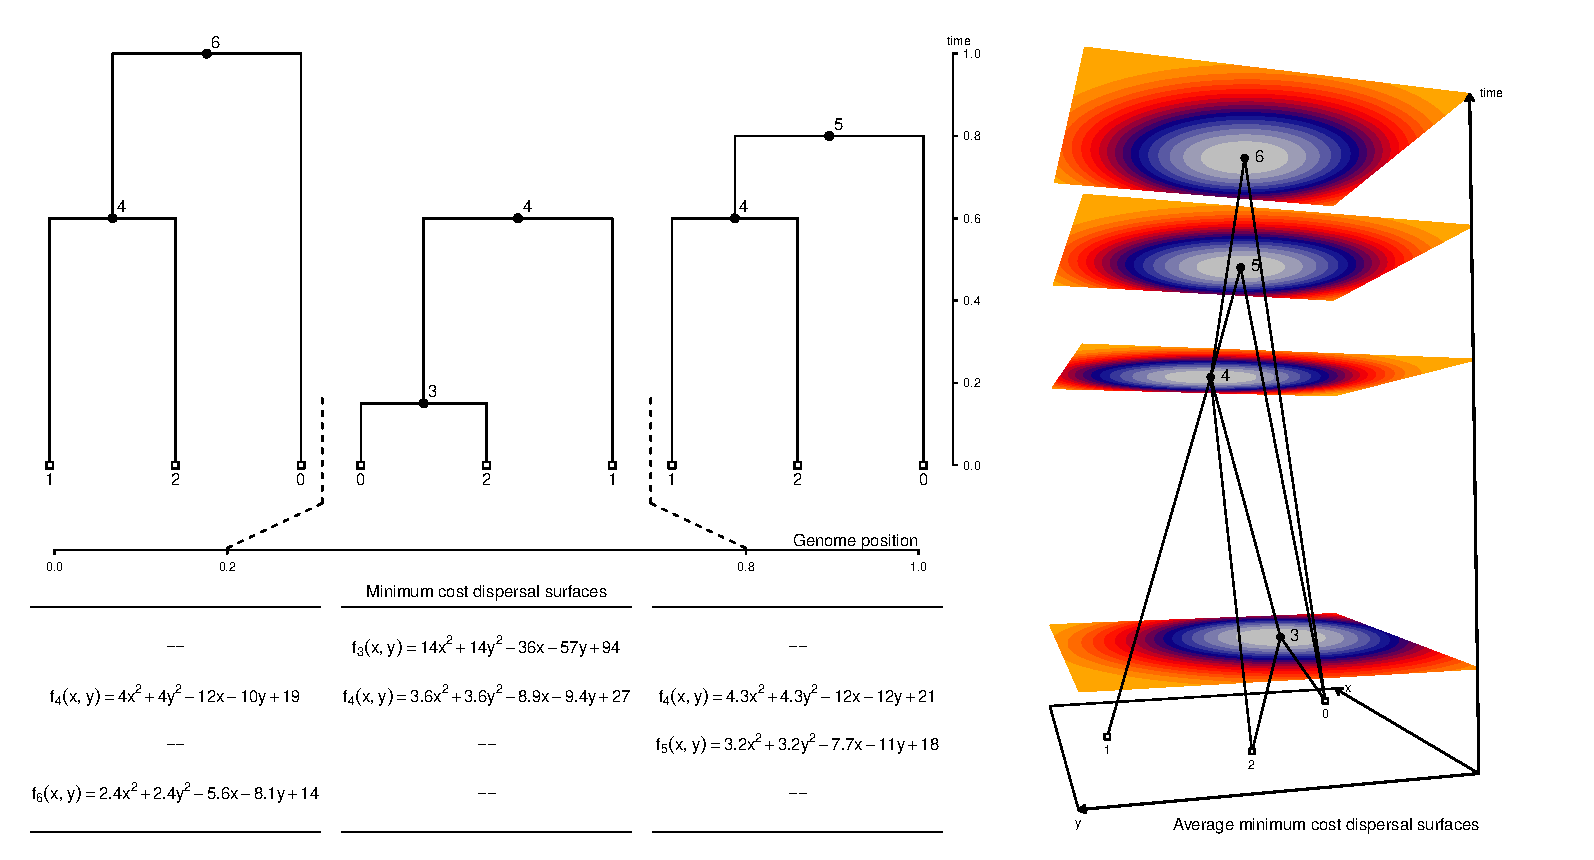
\includegraphics[width=\textwidth]{figs/concept-fig.pdf}}
% Pick an appropriate width - in print, figures are usually one or two columns wide, which can
% be approximated by 0.3\textwidth or 0.6\textwidth respectively. Use appropriate label sizes.

\caption{\textbf{Conceptual overview of \textsc{gaia}}. For each local tree we use the 
dynamic programming method of \cite{Sankoff_Rousseau_1975} to fit a 
minimum cost dispersal surface to the genealogical relationships of the 
georeferenced sample nodes. In this example, we use squared Euclidean 
distance as the cost function and $f_u(x,y)$ returns the smallest sum of 
squared dispersal distances between all ancestor-descendant node pairs 
that can be obtained when node $u$ is at location $(x,y)$. Using the 
genomic spans of local trees as weights, we then take a weighted average 
of local surfaces to assign each node a single average minimum cost 
dispersal surface. Here, node 4 appears in all three local trees and its 
final fitted surface is the weighted average of the three local surfaces. 
By contrast, nodes 3, 5, and 6 appear in a single local tree and their 
final fitted surfaces are identical to the surface in the local tree 
in which they appear. The perspective plot in the rightmost panel 
displays the ancestral recombination graph encoding the local trees 
along with the final fitted surface for each node. Non-sample nodes are 
positioned at the minimum cost point on the surface (warmer colors 
denote higher costs).}
\label{fig:concept}

\end{figure}


\begin{figure}
\centering
{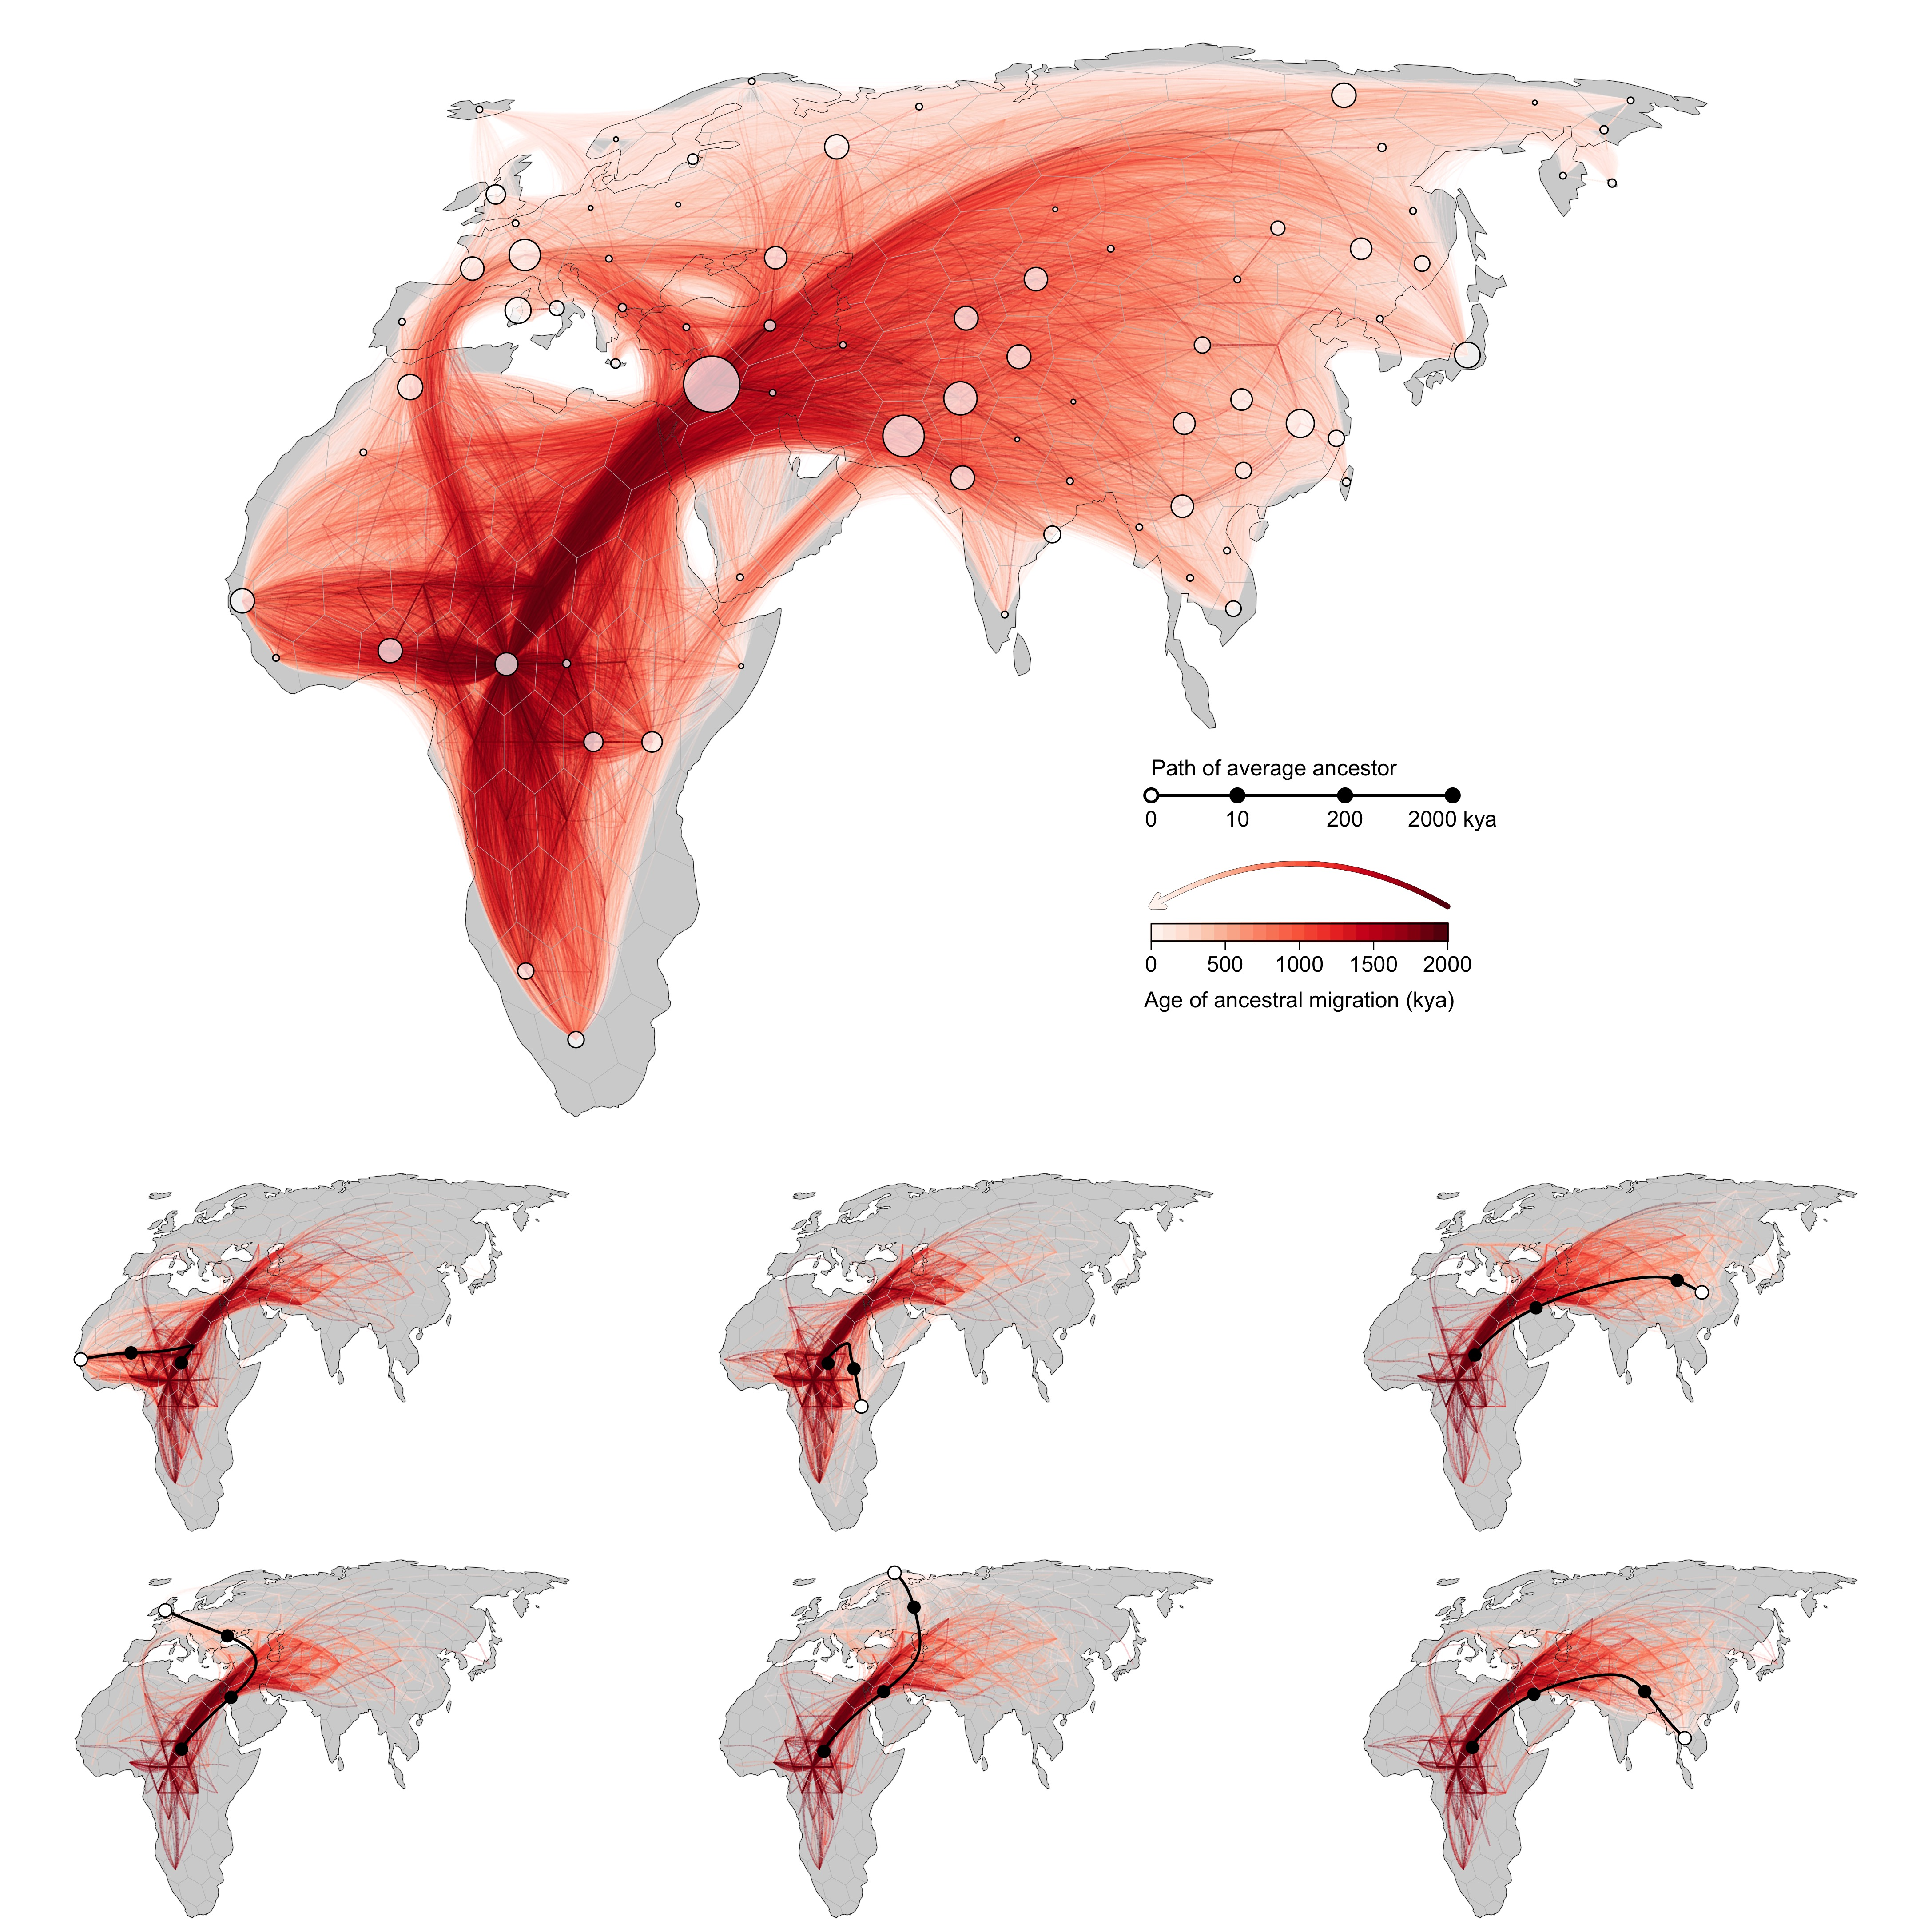
\includegraphics[width=\textwidth]{figs/tanglegram.jpg}}

\caption{\textbf{A georeferenced ancestral recombination graph (ARG)}. Red lines
trace the inferred historical migrations of genetic ancestors of the
sample (white points), with darker shading used to indicate movements 
that took place in the more distant past. Six contemporary samples are 
highlighted in the lower panels; black lines trace the average 
position of their genetic ancestors back through time, while red 
lines denote the subset of edges in the ARG that are ancestral to the 
samples.
}
\label{fig:tanglegram}

\end{figure}

\begin{figure}
\centering
{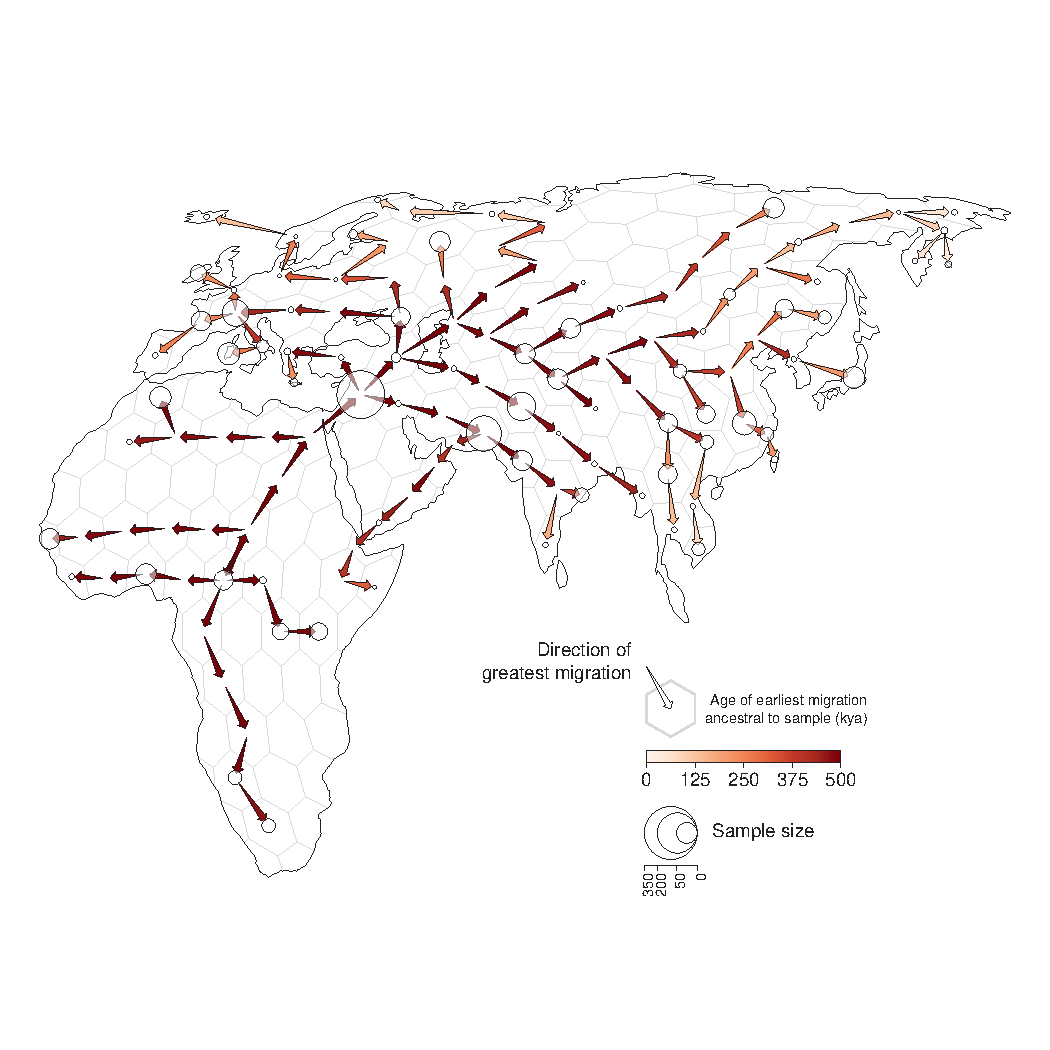
\includegraphics[width=\textwidth]{figs/overall-flux.pdf}} 

\caption{\textbf{Geographic chronology of human genetic ancestry}. Arrows
point in the direction of greatest migration of the shared genetic
ancestors of the sample and are colored according to the age of the
earliest migration. Points show the distribution of sampled modern-day 
genomes. Point size is proportional to the number of samples from each 
locality.}
\label{fig:overall}

\end{figure}

\begin{figure}
\centering
{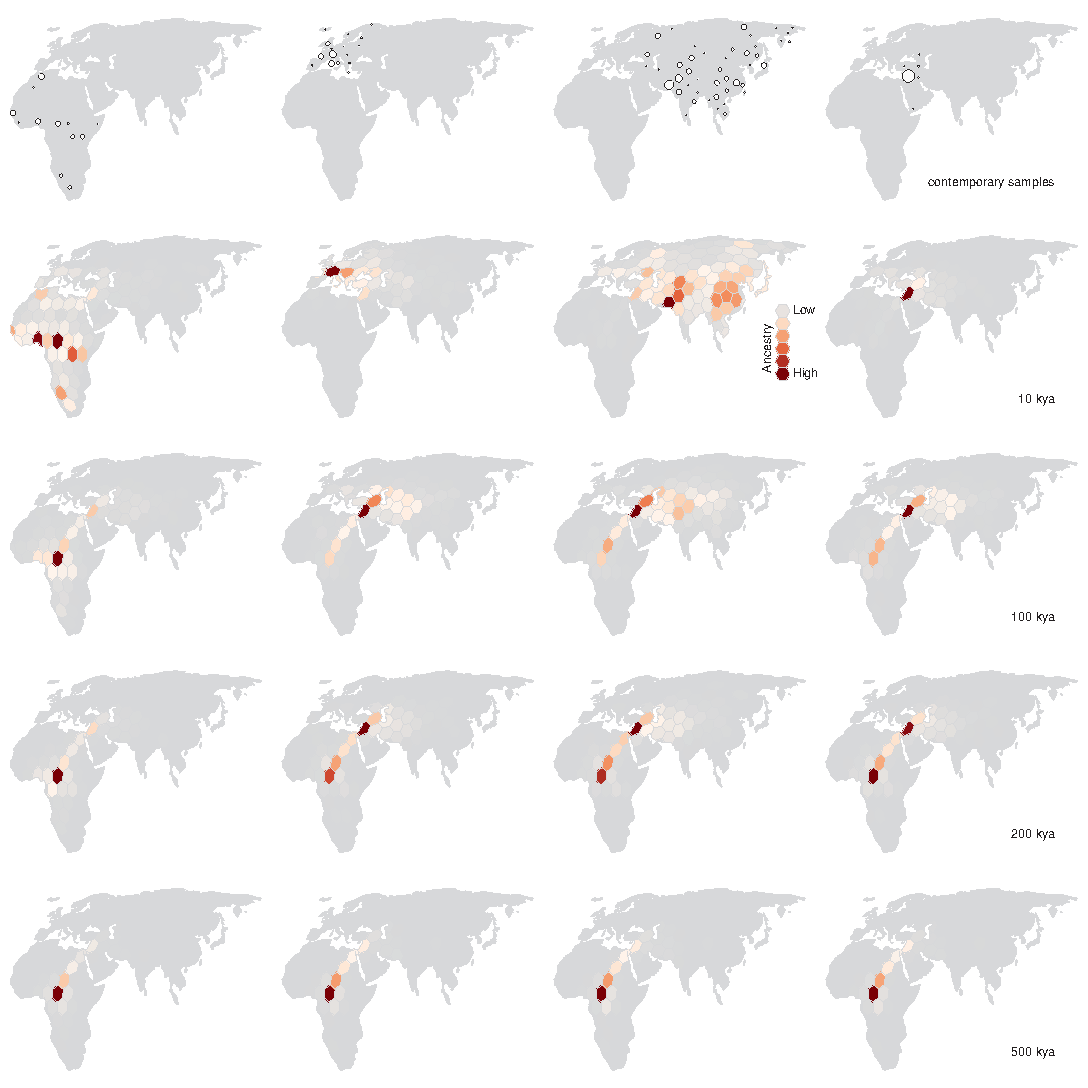
\includegraphics[width=\textwidth]{figs/ancestry-thru-time.pdf}} 

\caption{\textbf{Inferred spatiotemporal ancestry coefficients through time}.
The fraction of genomic positions in each geographic subset of 
samples (top row) that trace ancestry to different geographic regions at
different times in the past is represented by shades of red, with
darker shading indicating greater ancestry (=a larger fraction). 
Point size is proportional to the number of sampled genomes from each 
locality.
}
\label{fig:ancestry}

\end{figure}

\begin{figure}
\centering
{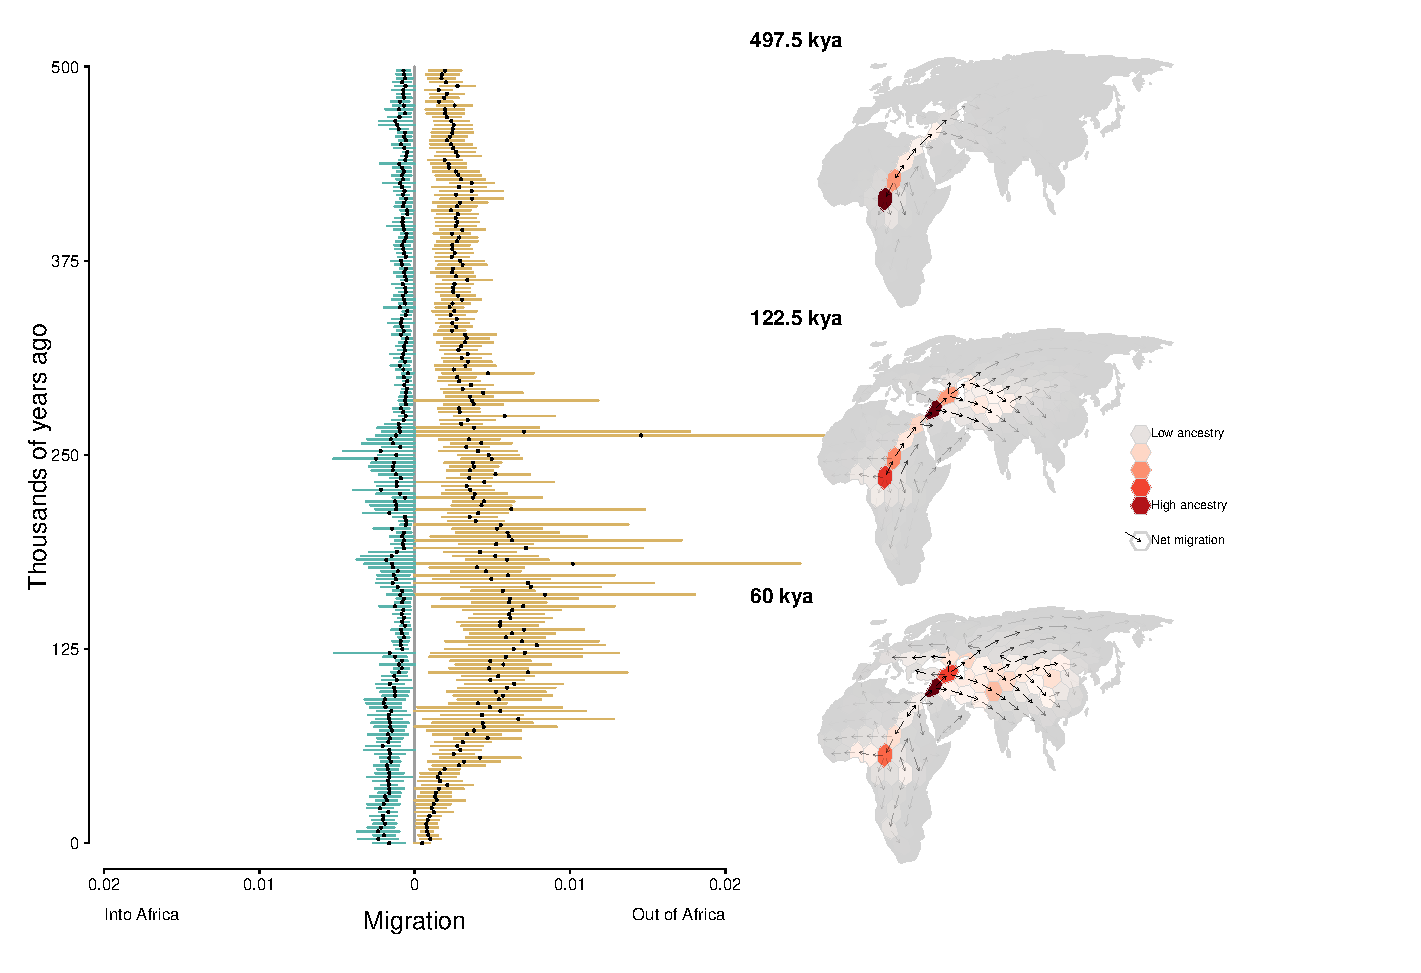
\includegraphics[width=\textwidth]{figs/ooa-flux.pdf}}   

\caption{\textbf{Inferred flux in spatiotemporal ancestry coefficients through
time}. Each point is the mean estimate (computed from random subsets of the data
and bracketed by the standard deviation) of the amount of historical migration 
of shared genetic ancestors of the modern-day sample into or out of Africa over 
time. Inset maps highlight three different time intervals. Cells are colored by 
the fraction of genomic positions that find ancestry in them at that time and arrows
depict the direction of greatest migration with opacity scaled by the
magnitude migration.}
\label{fig:ancestry-flux}

\end{figure}

%%%%%%%%%%%%%%%% MAIN TEXT TABLES %%%%%%%%%%%%%%%


%%%%%%%%%%%%%%%% REFERENCES %%%%%%%%%%%%%%%

\clearpage % Clear all remaining figures and tables then start a new page

% The list of references goes after the main text and before the acknowledgements
% When preparing an initial submission, we recommend you use BibTeX, like this:
%
\bibliography{gaia.bib} % for a file named science_template.bib
\bibliographystyle{sciencemag}

% After the paper has completed peer review and been revised ready for acceptance,
% you should comment out the lines above and copy-paste the contents of your .bbl
% file here instead. This will help ensure that our conversion software works correctly.
% Remember to re-run BibTeX first - check the timestamp!
%
% Example of the first three entries copy-pasted from science_template.bbl:
%
%\begin{thebibliography}{1}
%
%\bibitem{example}
%A.~N. {Author}, An example reference. \emph{Journal of Improbable Research}
%  \textbf{1}, 67 (2020).
%
%\bibitem{example2}
%F.~M. {Surname}, S.~{Author}, A second example. \emph{Interesting Research
%  Letters} \textbf{32}, 897 (2019).
%
%\bibitem{example_preprint}
%P.~{One}, P.~{Two}, P.~{Three}, {An unpublished preprint}. \emph{preprint}
%  (2021), arXiv:2101.12345.
%
%\end{thebibliography}


%%%%%%%%%%%%%%%% ACKNOWLEDGEMENTS %%%%%%%%%%%%%%%

\section*{Acknowledgments}
We thank Yaniv Brandvain, Jed Carlson, Graham Coop, Puneeth Deraje, Doc Edge,
James Kitchens, Marjorie Weber, and members of the Bradburd lab for comments
and discussion that helped improve the research presented here.
\paragraph*{Funding:}
This research was supported by the National Science Foundation (award number
DMS-2052653 to JT) and the National Institute of General Medical Sciences of the
National Institutes of Health under award numbers R35GM151145 (JT) and
R35GM137919 (GSB). The content is solely the responsibility of the authors and
does not necessarily represent the official views of the National Institutes of
Health.
\paragraph*{Author contributions:}
\textbf{MCG}: Conceptualization, Methodology, Software, Validation, 
Formal analysis, Data Curation, Writing - Original Draft, Writing - Review \&
Editing. \textbf{JT}: Conceptualization, Methodology, Funding acquisition,
Writing - Review \& Editing. \textbf{GSB}: Conceptualization, Methodology, 
Funding acquisition, Supervision, Writing - Original Draft, 
Writing - Review \& Editing.
\paragraph*{Competing interests:}
There are no competing interests to declare.
\paragraph*{Data and materials availability:} 
All publicly available datasets used in this paper are available from their
original publications. \textsc{gaia} is available at
\url{https://github.com/blueraleigh/gaia} under the MIT License. All code and data
files used to perform analyses in this paper are available on GitHub at
\url{https://github.com/blueraleigh/gaia-paper} and on Dryad at
\url{https://doi.org/10.5061/dryad.p5hqbzkwz}.

%%%%%%%%%%%%%%%% SUPPLEMENT LIST %%%%%%%%%%%%%%%

% List the contents of your Supplementary Materials, including the numbers of any
% supplementary figures, tables, external data files etc. and any references that are
% cited only in the supplement. In this example, refs. 7-8 are cited only in the supplement.
% Fill out your numbers accordingly and delete any lines that aren't applicable.
\subsection*{Supplementary materials}
Materials and Methods\\
Supplementary Text\\
Figs. S1 to S14\\
References \textit{(37-\arabic{enumiv})} % automatically fills out the last reference number
% (filling out the other numbers automatically is possible but fiddly and liable to break)


%%%%%%%%%%%%%%%% END OF MAIN TEXT %%%%%%%%%%%%%%%

\newpage

%%%%%%%%%%%%%%%% START OF SUPPLEMENT %%%%%%%%%%%%%%%

% Figures, tables, equations and pages in the supplement are numbered S1, S2 etc.
\renewcommand{\thefigure}{S\arabic{figure}}
\renewcommand{\thetable}{S\arabic{table}}
\renewcommand{\theequation}{S\arabic{equation}}
\renewcommand{\thepage}{S\arabic{page}}
\setcounter{figure}{0}
\setcounter{table}{0}
\setcounter{equation}{0}
\setcounter{page}{1} % not 0 as \newpage already started a supplementary page
% References continue the numbering from the main text.

%%%%%%%%%%%%%%%% SUPPLEMENT TITLE PAGE %%%%%%%%%%%%%%%

\begin{center}
\section*{Supplementary Materials for\\ \scititle}

% Author list for the supplement
% Indicate the corresponding authors, but do NOT include institutions here
% It would be nice if the template auto-generated this, but doing so is complicated...
Michael~C.~Grundler,
Jonathan~Terhorst,
Gideon~S.~Bradburd$^{\ast}$\\ % we're not in a \author{} environment this time, so use \\ for a new line
\small$^\ast$Corresponding author. Email: bradburd@umich.edu
\end{center}

% Fill out the numbers for each type of supplementary material,
% and delete any lines that aren't applicable.
% These are just example numbers that don't match the rest of this template.
\subsubsection*{This PDF file includes:}
Materials and Methods\\
Supplementary Text\\
Figures S1 to S14

\newpage

%%%%%%%%%%%%%%%% MATERIALS AND METHODS %%%%%%%%%%%%%%%

\subsection*{Materials and Methods}

\subsubsection*{Main approach: computing minimum migration fits to local trees}

Given a set of sampled genomes with known locations and a tree sequence that
relates the samples, \textsc{gaia} efficiently reconstructs the locations of
genetic ancestors using a minimum migration heuristic. Conceptually, \textsc{gaia}
may be thought of as proceeding in three steps (Fig.~\ref{fig:concept}).

In the first step, a minimum migration cost function $f_{uk}$ is fitted to each
node $u$ in each local tree $k$ in which $u$ appears using the generalized
parsimony algorithm~\cite{Sankoff_1975, Sankoff_Rousseau_1975}. For each
spatial location, $f_{uk}(x)$ then returns the smallest sum of migration costs
between all ancestor-descendant pairs in local tree $k$ that can explain the
sampled locations when $u$ is at location $x$. We assume migration cost is a
function of migration distance and provide three cost function implementations.
In each of these three cases we allow migration distances to optionally be
weighted by inverse branch length. For a continuous state space, we use either
the squared Euclidean distance or the Manhattan distance. Squared Euclidean
distance leads to cost functions that are convex quadratic functions of the
spatial locations~\cite{Maddison_1991}; Manhattan distance, to convex piecewise linear functions
~\cite{Csuros_2008}. For a finite set of geographic locations, a square matrix
with arbitrary transition costs between all pairs of geographic states leads
to minimum migration costs that are discrete functions defined on the set of
geographic locations~\cite{Clemente_etal_2009}.

In the second step, we form a new function $F_u$ by taking a weighted average of
$f_{uk}$ over the local trees in which $u$ appears, using the genomic spans of
each local tree as weights. We interpret $F_u$ as the minimum migration cost of
an average ancestral base pair. In other words, if one were to take each
sampled base pair that inherits from $u$ and fit a minimum migration cost
function to its coalescent history, the average of those would look like $F_u$.
In the Supplementary Text, we present a detailed description of the algorithm we use for
computing $F_u$ from the local tree fits $f_{uk}$. Considerable computational
savings can be achieved by using the succinct tree sequence encoding
\cite{Kelleher_etal_2016}, which allows us to efficiently maintain the state of
parsimony calculations as we iterate over local trees. As detailed in the
Supplementary Text, the local tree fits also allow us to compute an estimate of
effective migration rate, which we define as the mean lineage migration cost
of an average base pair. That is, if one were to take the coalescent history
of each sampled base pair and compute the mean the per-branch migration cost
in a most parsimonious migration history, the average of those -- taken over
all sampled base pairs -- would equal the effective migration rate.

Finally, we locate each ancestor by finding the spatial location $x$ where $F_u
(x)$ is smallest. A constrained (rather than global) minimization of $F_u$
could also be used to locate ancestors if some spatial locations are known to
be uninhabitable. Although we do not pursue this possibility in the current
study, uncertainty in ancestor locations could be explored by sampling from
$\exp\bigl(-\lambda [F_u(x) - \min_z F_u(z)]\bigr)$, where $\lambda$ is a tuning 
parameter that controls how strongly deviations from the spatial location that 
minimizes the overall migration cost are penalized.

\subsubsection*{Spatiotemporal ancestry coefficients}

We use our ancestor location estimates to define two spatially and temporally
explicit ancestry coefficients as follows. In the first case, consider a subset
$i$ of the sampled genomes. Define $A_i(t)$ to be the total amount of sample
material in the subset that is descended from ancestral material at a point in
time $t$ in the past. Define $A_{ik}(t)$ to be the total amount of sample
material descended from ancestral material in geographic location $k$ at time $t$
in the past. We then define the spatiotemporal ancestry coefficient for subset
$i$ as $z_{ik}(t) = \frac{A_{ik}(t)}{A_i(t)}$, the fraction of sample material
that is descended from ancestral material in geographic location $k$ at time $t$
in the past. Thus, if we were to pool all sample material in subset $i$ whose
coalescent history extended at least $t$ time units into the past, $z_{ik}
(t)$ is the probability that we can trace the coalescent history of a randomly
selected base pair from that pool to an ancestral base pair in geographic location
$k$ at time $t$ in the past.

Next, define $A_i(t_l,t_r)$ to be the total amount of sample material in the
subset that is descended from ancestral material present during an interval in
time $[t_l,t_r)$ in the past. Define $A_{ijk}(t_l,t_r)$ to be the total amount
of sample material descended from ancestral material that migrated from
geographic location $j$ to location $k$ during an interval in time $[t_l, t_r)$ in
the past (where $j$ is not equal to $k$). We then define the spatiotemporal
ancestry flux coefficient for subset $i$ as $\phi_{ijk}(t_l, t_r) = \frac{A_
{ijk}(t_l, t_r)}{A_i(t_l, t_r)}$. Thus, if we were to pool all sample material
in subset $i$ whose coalescent history extended at least $[t_l,t_r)$ time units
into the past, $\phi_{ijk}(t_l,t_r)$ is the probabily that we can trace the
coalescent history of a randomly selected base pair from that pool to an
ancestral base pair that migrated from geographic location $j$ to location $k$ during
the interval $[t_l,t_r)$ in the past.

As defined, our spatiotemporal ancestry coefficients require knowing the
geographic locations of ancestral lineages at arbitrary points in time in the
past but our minimum migration location estimates (i.e., $\arg\min_x F_u
(x)$) are available only for the two endpoints of an ancestral lineage. By
using the migration cost function and conditioning on these endpoint states,
however, we can sample a minimum cost migration history for each lineage and
linearly interpolate the history between the endpoint times of the ancestral 
lineage. In this way we can locate ancestors at arbitrary points in time.


\subsubsection*{Simulation study: testing ancestor location accuracy}

We tested performance of \textsc{gaia} using spatially explicit forward-time
simulations in SLiM v4.0.1~\cite{Haller_Messer_2023}. Simulated individuals
were semelparous and hermaphroditic and diploid for a single chromosome with
$10^8$ basepairs and a recombination rate of $10^{-8}$ per basepair per
generation. Individuals coexisted on a two-dimensional square plane with
reflecting boundaries and a side length of $1000\sigma$ units, where $\sigma$
was the standard deviation of the dispersal kernel.

Population regulation occurred via density dependent effects on fecundity and
survival. The number of offspring produced by a focal individual in generation
$t$ was Poisson-distributed with a mean equal to $\frac{R}{1 + \frac
{N_t \times (R-1)}{K}}$, where $N_t$ is the local population density in a
circle of radius $3\sigma$ around the focal individual at generation $t$, $R$
is the population growth rate at low density, and $K$ is the local carrying
capacity density. During reproduction, each individual (the ``mother") chose a
mate (the ``father") uniformly at random from the set of individuals living
within a radius of $3\sigma$ from itself. A random location centered on the
mother's location was then chosen for each offspring by drawing from a
dispersal kernel with a standard deviation of $\sigma$. Each offspring produced
in generation $t$ survived to reproduce in generation $t+1$ with probability
$\min(1.0, \frac{K}{O_t})$, where $O_t$ is the local population density in a
circle of radius $3\sigma$ around the focal offspring in generation $t$.

We conducted simulations using either a Gaussian dispersal kernel or a double
exponential dispersal kernel and 10 different $\sigma$ levels that were equally
spaced from 0.2 to 2.0. The Gaussian kernel emulates a Brownian motion while
the double exponential kernel emulates a Laplace motion, which generates more
extreme displacements of offspring relative to Brownian motion.

We conducted 10 replicate simulations for each $\sigma$ level under each
dispersal kernel. For all simulations, we set $R=2$ and $K=\frac{30}{
(3\sigma)^2\pi}$. Each simulation was initiated from a randomly located founder
population of 30 individuals that was allowed to grow and disperse for 10,000
generations, after which the simulation was terminated and the recorded
(simplified) tree sequence of extant individuals was saved for analysis.

Simulations conducted under the Gaussian dispersal kernel were analyzed using
squared Euclidean distance weighted by inverse branch length as the transition
cost function. Simulations conducted under the double exponential dispersal
kernel were analyzed using Manhattan distance weighted by inverse branch length
as the transition cost function. For all simulations we evaluated our ability
to accurately estimate effective migration rates and the locations of genetic
ancestors. We defined the true effective migration rate ($\sigma_e$) to be the
maximum likelihood estimate of $\sigma$ under each dispersal kernel assuming we
had complete knowledge of the locations of all ancestral individuals in the
tree sequence.

To explore how robust \textsc{gaia} may be to deviations from isotropic dispersal,
we carried out a further set of simulations where carrying capacity was not 
constant across the landscape. Instead, local carrying capacity varied over space 
according to a stationary Gaussian random field with a mean of 30 (the same
constant limit as the previous simulations) and a marginal variance of 40. Each 
simulation was initiated from 300 uniformly chosen localities and each locality 
was seeded with 30 individuals. Details of simulated individuals
and population regulation were identical to the simulations discussed above.
We conducted simulations using either a Gaussian dispersal kernel with a
standard deviation of $\sigma=0.025$ or a Pareto dispersal kernel with a minimum
offspring dispersal distance of $\sigma=0.025$ and with an infinite variance
(corresponding to a shape parameter of 2). As before, each simulation landscape
was a two-dimensional square plane with reflecting boundaries and a side length 
of $1000\sigma$ units. Twenty replicate simulations were conducted with 
each dispersal kernel, and each simulation was allowed to run for
10,000 generations, after which the simulation was terminated and the recorded
tree sequence of extant individuals was saved for analysis with \textsc{gaia}
using squared Euclidean distance weighted by inverse branch length as the 
transition cost function.

For all simulations we compare ancestor location inferences from \textsc{gaia}
to corresponding inferences from the non-parametric method introduced by
~\cite{Wohns_etal_2022}.


\subsubsection*{Empirical example: reconstructing human migration out of Africa}

We applied \textsc{gaia} to a contemporary sample of georeferenced human
genomes from the Human Genome Diversity Project using the dated tree sequence
inferred for the short arm of chromosome 18 by~\cite{Wohns_etal_2022}. Prior to analysis, we
first simplified the tree sequence to include only individuals from Africa,
Asia, and Europe. Certain non-sample nodes in the tree sequence are clear
outliers with respect to the number of edges in which they participate. For example,
one node has nearly 3,000 immediate descendants, well above the median number
of 6. As these genealogical outliers have the potential to strongly bias
geographic reconstructions, we further simplified the tree sequence by removing 
edges to or from non-sample nodes in the upper two percent of in-degree or 
out-degree counts. The resulting simplified tree sequence consisted of 28,154 
local genealogies, containing 114,606 ancestral nodes and spanning approximately 
80,000 generations of human history.

To explore historical geographic patterns in human genetic ancestry over the
last one-half million years we created a set of equal-interval time bins
spanning 100 generations (or 2,500 years using a 25 year generation time) that
extended from the present to 20,000 generations in the past. An equal area
discrete global grid~\cite{Barnes_Sahr_2023} (cell spacing approximately 800 
km) intersected with Earth's landmass provided a set of habitable locations.
Individual samples were then mapped to the nearest grid cell and we used
\textsc{gaia} to compute $F_u$ for each node in the empirical tree sequence
using a simple cost matrix that assigned a unit cost to each migration event
and only allowed migration between neighboring grid cells.

Each internal node in the tree sequence was then geographically referenced by
sampling uniformly at random one of the grid cells that minimized its migration
cost function $F_u$ (for some nodes there may be a unique grid cell that
achieves this minimum but for others there may be multiple). This procedure was 
repeated 100 times and spatiotemporal ancestry coefficients were computed for
each realization and then averaged.

To ensure our results were robust to sampling variation, we repeated all
analyses on 100 random subsets of the data. Data were subsetted so that each 
identified population in the dataset was represented by a single individual and
the tree sequence was then simplified to include only the subsetted individuals.
We chose to subset individuals within identified populations rather
than within grid cells to maximize the amount of genetic diversity retained in
the simplified tree sequence. Any subsetting procedure will prune branches from 
the tree sequence. Depending on the phylogenetic position of pruned branches, 
their loss can be consequential for tree-based inference methods like
\textsc{gaia}. In particular, the loss of deep-rooted branches will impact
ancestor inferences more than the loss of shallow-rooted branches. Of course, 
these same concerns also apply to the original sampling design and we should be
cautious about any inferences from datasets suspected of missing substantial 
amounts of extant genetic diversity.

In an effort to determine some of the limits of \textsc{gaia} inference with
the empirical sampling distribution and assumed transition cost function, 
we conducted a set of SLiM simulations on the same discrete representation of 
Earth's landmass that we used for the empirical analysis. Simulated individuals were either male or female,
and diploid for a single chromosome with $10^8$ basepairs and a recombination 
rate of $10^{-8}$ per basepair per generation. Density-independent survival
was 0.6 in the first two years of life and then 0.95 until age 55,
after which survivorship declined linearly to zero at age 80. Each grid cell 
corresponded to a panmictic subpopulation with a carrying capacity of 100.
Each subpopulation exchanged sexually mature migrants with its neighboring subpopulations 
at a rate of 0.001. Individual females were capable of mating and giving birth to a single
offspring from age 15 to age 40, and individual males could mate from age 15 to age 55.
We conducted 75 replicate simulations, starting each simulation from a single
subpopulation in eastern Africa. In 25 of the simulations, dispersal out of
Africa could occur only across the Sinai peninsula; in another 25 simulations,
dispersal could occur only across the strait at Bab-el-Mandeb; in the final
25 simulations, dispersal out of Africa could occur using both routes. We
analyzed all simulations with \textsc{gaia} assuming dispersal could occur
via either route of Africa and assuming a unit cost for each migration between
grid cells. Prior to analysis with \textsc{gaia}, we simplified all recorded
tree sequences to retain just a single individual from each grid cell for which
individuals were sampled in empirical dataset.

%%%%%%%%%%%%%%%% SUPPLEMENTARY TEXT %%%%%%%%%%%%%%%

\subsection*{Supplementary Text}


\subsubsection*{\textsc{gaia}'s use of generalized parsimony}

We first review generalized parsimony as it applies to a single gene tree
~\cite{Sankoff_1975, Sankoff_Rousseau_1975}. For each node $u$ we maintain
three cost functions. The \textit{node cost} function $g_u(x)$ assigns a cost
to each geographic state $x$ (when $u$ is in state $x$) that gives the minimum
migration cost required to explain the geographic states of all sample nodes
whose most recent common ancestor is $u$. If $u$ is a sample node, we set
$g_u(x) = 0$ if $x = x_u$ and $g_u(x) = \infty$ if $x \neq x_u$. When $u$ is 
not a sample node, $g_u$ is formed by the sum of the \textit{stem cost}
functions of its children.

The stem cost function for a node $u$ is given by
%
$h_u(x) = \min_z \bigl[ \Delta_u(x, z) + g_u(z) \bigr]$.
%
The function $\Delta_u(x, z)$ assigns a cost to the migration from state $x$ to
state $z$ over the branch leading to node $u$. Here, we assume that $\Delta_u$
can be factored as:
%
$\Delta_u(x,z) = \phi(\tau_u) * \Delta(x,z)$,
%
where $\tau_u$ is the length of the branch leading to node $u$ and $\Delta$ is
a time-independent transition cost function. Typical choices for the
time-dependent component are $\phi(\tau_u) = \frac{1}{\tau_u}$ or 
$\phi(\tau_u) = 1$, the latter making the whole cost function independent of
branch lengths.

The node cost and stem cost functions can be computed in a single post-order
tree traversal. A second pre-order tree traversal can then be used to compute
the \textit{final cost} functions for each node. The final cost $f_u(x)$
gives the minimum migration cost required to explain the geographic states of
\emph{all} sample nodes when $u$ is in state $x$. When $u$ is the root of the
tree, $f_u(x) = g_u(x)$. Otherwise, 
%
$f_u(x) = \min_z \bigl[ f_{\pi_u}(z) - h_u(z) + \Delta_u(z,x) \bigr] + g_u(x)$,
%
where $\pi_u$ represents the immediate ancestor of node $u$ \cite{Clemente_etal_2009}.

In our implementation, $x$ can either be a coordinate vector in a 
continuous multidimensional space or a scalar integer that indexes a set of discrete
geographic locations. If the former, \textsc{gaia} can compute cost functions
using squared-change \cite{Maddison_1991} and linear parsimony \cite{Csuros_2008}.
In the case of squared-change parsimony, all cost functions are convex quadratic
functions whose parameters can be calculated analytically for each node in $\mathcal{O}(1)$ time.
In the case of linear parsimony, all cost functions are convex piecewise linear
functions whose parameters can be calculated analytically for each node in at most 
$\mathcal{O}(n)$ time, where $n$ is the number of samples in the tree sequence.
If the geographic space is discrete, \textsc{gaia} computes cost functions for each node in
$\mathcal{O}(n^2)$ time, where $n$ is the number of geographic states~\cite{Clemente_etal_2009}.


\subsubsection*{\textsc{gaia}'s use of succinct tree sequences}

Here we describe how we use the succinct tree sequence encoding
\cite{Kelleher_etal_2016} to efficiently compute node cost and stem cost 
functions for each local genealogy. Under the coalescent with recombination, 
nearby gene trees are highly correlated. Moving between adjacent local trees 
typically requires only a small number of subtree-prune-and-regraft (SPR) 
operations. By keeping an index of the edges involved in these SPR operations 
and the order in which they need to be applied, the succinct tree sequence 
encoding allows us to efficiently maintain the state of parsimony calculations 
as we iterate over the local genealogies.

A detailed description of the tree sequence data structure can be found in
\cite{Kelleher_etal_2016}. For our purposes, it suffices to know that
relationships among all $N$ nodes in the tree sequence are recorded in the edge 
table $E$. Each row in the edge table records an ancestor-descendant
relationship, and the indices of nodes involved in that relationship can be 
accessed as $E[k].\texttt{parent}$ and  $E[k].\texttt{child}$. The relationship 
encoded by an edge applies to the half-open genomic interval between $E[k].\texttt{left}$ 
(inclusive) and $E[k].\texttt{right}$ (exclusive). As we move along the genome 
from left to right, the index vectors $I$ and $O$ give the insertion and
removal order of the edges needed to build each local gene tree topology 
(recorded in the vector $\pi$: $\pi_u$ is the immediate ancestor of node $u$). 
The following algorithm is based on the branch statistic algorithm that appears 
in \cite{Ralph_etal_2020} but differs in its treatment of sample weights and 
how they are propagated along a genealogy.

\subsubsection*{Algorithm P (generalized parsimony)}

Given a set of georeferenced samples related by a tree sequence with length
$L$, compute the genome-wide average final cost function $F_u(x)$ and the
genome-wide average migration rate statistic $\sigma_P$. The function $F_u(x)$ 
returns the average minimum migration cost required to explain the observed 
geographic states of all sample nodes when $u$ is in state $x$, where the 
average is taken over all local genealogies (weighted by their genomic span)
where node $u$ appears. The statistic $\sigma_P$ is the average per-branch 
migration cost in a most parsimonious migration history averaged over all
local genealogies weighted by their genomic span. Note that the specific 
form of $F_u(x)$ will depend on the nature of the cost function
and geographic state, which is used here in an abstract sense (it may be 
continuous or discrete).

Local variables include the edge loop counters $j$ and $k$; the node indices
$u$, $v$, and $w$; the left and right genomic coordinates, $t_l$ and $t_r$, of 
the current local tree, as well as their difference $s$, recording the genomic 
span of the tree; the variable $s_u$ keeps track of the total genomic span of 
node $u$, which is needed for efficiently computing $F_u(x)$; the variable $s_P$ 
keeps track of the cumulative genomic span already visited and is used together 
with $\sigma$, the minimum migration cost of the current local tree, to 
efficiently compute $\sigma_P$.

\begin{description}

\item[S1.] [Initialization.]
    For $0 \leq u < N$
        set $\pi_u \leftarrow -1$,
        $s_u \leftarrow 0$,
        $g_u(x) \leftarrow 0$,
        $F_u(x) \leftarrow 0$.
        Then,
        if $u$ is a sample node and $x \neq x_u$,
            set $g_u(x) \leftarrow \infty$ and $F_u(x) \leftarrow \infty$

    Finally,
        set $j \leftarrow 0$,
        $k \leftarrow 0$,
        $\sigma_P \leftarrow 0$,
        $t_l \leftarrow 0$,
        $s_P \leftarrow 0$.

\item[S2.] [Terminate.]
    If $j = |E|$ terminate.

\item[S3.] [Edge removal loop.]
    If $k = |E|$ or $t_l \neq E[O_k].\texttt{right}$ go to S6.

\item[S4.] [Remove edge.]
    Set $u \leftarrow E[O_k].\texttt{parent}$,
        $v \leftarrow E[O_k].\texttt{child}$,
        $w \leftarrow \pi_u$, and
        $k \leftarrow k + 1$.
        Then,
        if $w \neq -1$,
            set $g_w(x) \leftarrow g_w(x) - h_u(x)$.
        Finally,
        set $g_u(x) \leftarrow g_u(x) - h_v(x)$,
        $\pi_v = -1$,
        $v \leftarrow u$,
        $u \leftarrow w$.

\item[S5.] [Update node and stem costs.]
    While $u \neq -1$,
        set $w \leftarrow \pi_u$ and
        if $w \neq -1$
            set $g_w(x) \leftarrow g_w(x) - h_u(x)$.
        Then set
        $h_v(x) \leftarrow \min_{z}\bigl[\Delta_v(x,z) + g_v(z)\bigr]$,
        $g_u(x) \leftarrow g_u(x) + h_v(x)$,
        $v \leftarrow u$, $u \leftarrow w$.
    Afterward, go to S3.

\item[S6.] [Edge insertion loop.]
    If $j = |E|$ or $t_l \neq E[I_j].\texttt{left}$ go to S9.

\item[S7.] [Insert edge.]
    Set $u \leftarrow E[I_j].\texttt{parent}$,
        $v \leftarrow E[I_j].\texttt{child}$,
        $w \leftarrow \pi_u$, and
        $j \leftarrow j + 1$.
        Then,
        if $w \neq -1$,
            set $g_w(x) \leftarrow g_w(x) - h_u(x)$.
        Then set
        $h_v(x) \leftarrow \min_{z}\bigl[\Delta_v(x,z) + g_v(z)\bigr]$.
        Finally,
        set $g_u(x) \leftarrow g_u(x) + h_v(x)$,
        $\pi_v = u$,
        $v \leftarrow u$,
        $u \leftarrow w$.

\item[S8.] [Update node and stem costs.]
    While $u \neq -1$,
        set $w \leftarrow \pi_u$ and
        if $w \neq -1$
            set $g_w(x) \leftarrow g_w(x) - h_u(x)$.
        Then
        set $h_v(x) \leftarrow \min_{z}\bigl[\Delta_v(x,z) + g_v(z)\bigr]$,
        $g_u(x) \leftarrow g_u(x) + h_v(x)$,
        $v \leftarrow u$, $u \leftarrow w$.
    Afterward, go to S6.

\item[S9.] [Genomic span of tree.]
    Set $t_r \leftarrow L$.
    If $j < |E|$ set
        $t_r \leftarrow \min\bigl(t_r, E[I_j].\texttt{left}\bigr)$.
    Then,
    if $k < |E|$ set
        $t_r \leftarrow \min\bigl(t_r, E[O_k].\texttt{right}\bigr)$.
    Set $s \leftarrow t_r - t_l$.

\item[S10.] [Update average migration costs.]
    Set $\sigma \leftarrow 0$, $n \leftarrow 0$, $s_P \leftarrow s + s_P$.
    Then visit each node $u$ in a pre-order traversal and set
    $s_u \leftarrow s_u + s$.
    If $\pi_u = -1$ set
        $f_u(x) \leftarrow g_u(x)$ and set
        $\sigma \leftarrow \sigma + \min_z f_u(z)$;
    otherwise, set 
        $f_u(x) \leftarrow \min_z \bigl[ f_{\pi_u}(z) - h_u(z) + \Delta_u(z,x) \bigr] + g_u(x)$
        and set $n \leftarrow n + 1$.
    Then, set
        $F_u(x) \leftarrow F_u(x) + s \times \frac{f_u(x) - F_u(x)}{s_u}$.

\item[S11.] [Update average migration rate.]
    Set $\sigma_P \leftarrow \sigma_P + s \times \frac{\sigma/n - \sigma_P}{s_P}$.

\item[S12.] [Tree loop tail.]
    Set $t_l \leftarrow t_r$. Go to S2.

\end{description}

We begin in S1 by initializing the cost functions for each node to zero except in
the case of sample nodes, for which we set the cost function to positive infinity for all states
not equal to the observed state. We then set the parent of each node to $-1$ 
(signifying the null element) so that the initial state of the tree sequence
is a forest of disconnected nodes. The average cost functions (denoted by the
corresponding capital letters) are also initialized to $0$ as these will be
updated as we iterate over the tree sequence.

The meat of the algorithm occurs in steps S4 and S5 of the edge removal loop
and in steps S7 and S8 of the edge insertion loop. Removal of an edge from
node $u$ to $v$ will alter the node and stem cost functions along the path from
$u$ back to the root of the genealogy. Step S4 prepares for this by first
subtracting the stem costs of $u$ and $v$ from the node costs of their
respective parents. In step S5, we walk back along the path from $u$'s parent to
the root and recompute new stem costs and node costs given the updated node
costs at the head of the path. Insertion of an edge from node $u$ to $v$ will 
similarly alter the node and stem cost functions along the path from
$u$ back to the root of the genealogy. Step S7 prepares for this by first
substracting the stem cost of $u$ from the node cost of its parent and then
computing the stem cost of $v$ and adding it to the node cost of $u$. In step 
S8, we walk back along the path from $u$'s parent to the root as before and 
recompute new stem costs and node costs given the updated node costs at the 
head of the path.

Upon reaching step S9, we have finished constructing the tree together with its
node cost and stem cost functions. We record the genomic span of the tree in the 
variable $s$, which will be the weight applied to the current tree in the weighted
average. In S10, we perform a preorder traversal of the newly constructed tree
and compute the final cost function for each node. At the same time, we 
increment the total weight $s_u$ of each node by $s$ and update the weighted 
averages $F_u(x)$ with the cost functions for the current tree. When we begin
the traversal at the root(s) of the tree we also record the minimum migration 
cost $\sigma$ needed to explain the sample distribution. We use this cost in
S11, together with the number $n$ of edges in the tree, to update the weighted
average migration rate statistic $\sigma_P$.

Correctness of the algorithm requires that edges are removed in order of 
nondecreasing right genomic coordinate and decreasing time and that edges are
inserted in order of nondecreasing left genomic coordinate and increasing time
(time is measured backward from the present). We assume that the index vectors
$I$ and $O$ are constructed to satisfy these conditions; these assumptions 
form the basis of the conditional checks in steps S3 and S6 for determining
when to exit the edge removal and insertion loops.

\subsubsection*{Relation to existing work}

Several existing approaches to geographic inference with tree sequences merit 
discussion in relation to \textsc{gaia}. \cite{Wohns_etal_2022} introduced a
nonparametric approach that estimates ancestor locations by successively
averaging the coordinates of sample locations in a postorder traversal of the
ARG to their most recent common ancestor. The resulting estimates are local 
estimates in the sense that the inferred location of an ancestor depends only 
on the locations of samples that trace some portion of their ancestry to that 
ancestor and on the topology of the corresponding subset of the ARG. By contrast,
\textsc{gaia} estimates the location of an ancestor using information from all
samples. Because all samples share common ancestry at some time in the past, 
even those samples that are not direct descendants of an ancestor can be 
informative about that ancestor's location.

\cite{Osmond_Coop_2021} describe a likelihood method for locating genetic
ancestors and estimating migration rates that is based on a model of branching
Brownian motion. Their approach also uses information from all samples to
estimate ancestral locations and can optionally estimate separate migration
rates for deep and shallow time horizons. Unlike \textsc{gaia}, inference is 
carried out on a sample of widely spaced genealogies rather than on the full 
tree sequence. We note that when \textsc{gaia} is used with squared Euclidean distance weighted by inverse 
branch length as the transition cost function, the maximum parsimony 
reconstruction on each local genealogy has highest posterior probability 
under a Brownian motion dispersal process. In this sense, the genome-wide 
average reconstruction produced by \textsc{gaia} can be viewed as a weighted 
average of posterior modes. \cite{Deraje_etal_2024} recently extended the
model of branching Brownian motion to work with the full ARG rather than a
sample of local gene trees.

% If your supplement is very short you might need to uncomment the following line to avoid
% layout problems with the figures and tables.
\newpage

%%%%%%%%%%%%%%%% SUPPLEMENTARY FIGURES %%%%%%%%%%%%%%%


\begin{figure}
\centering
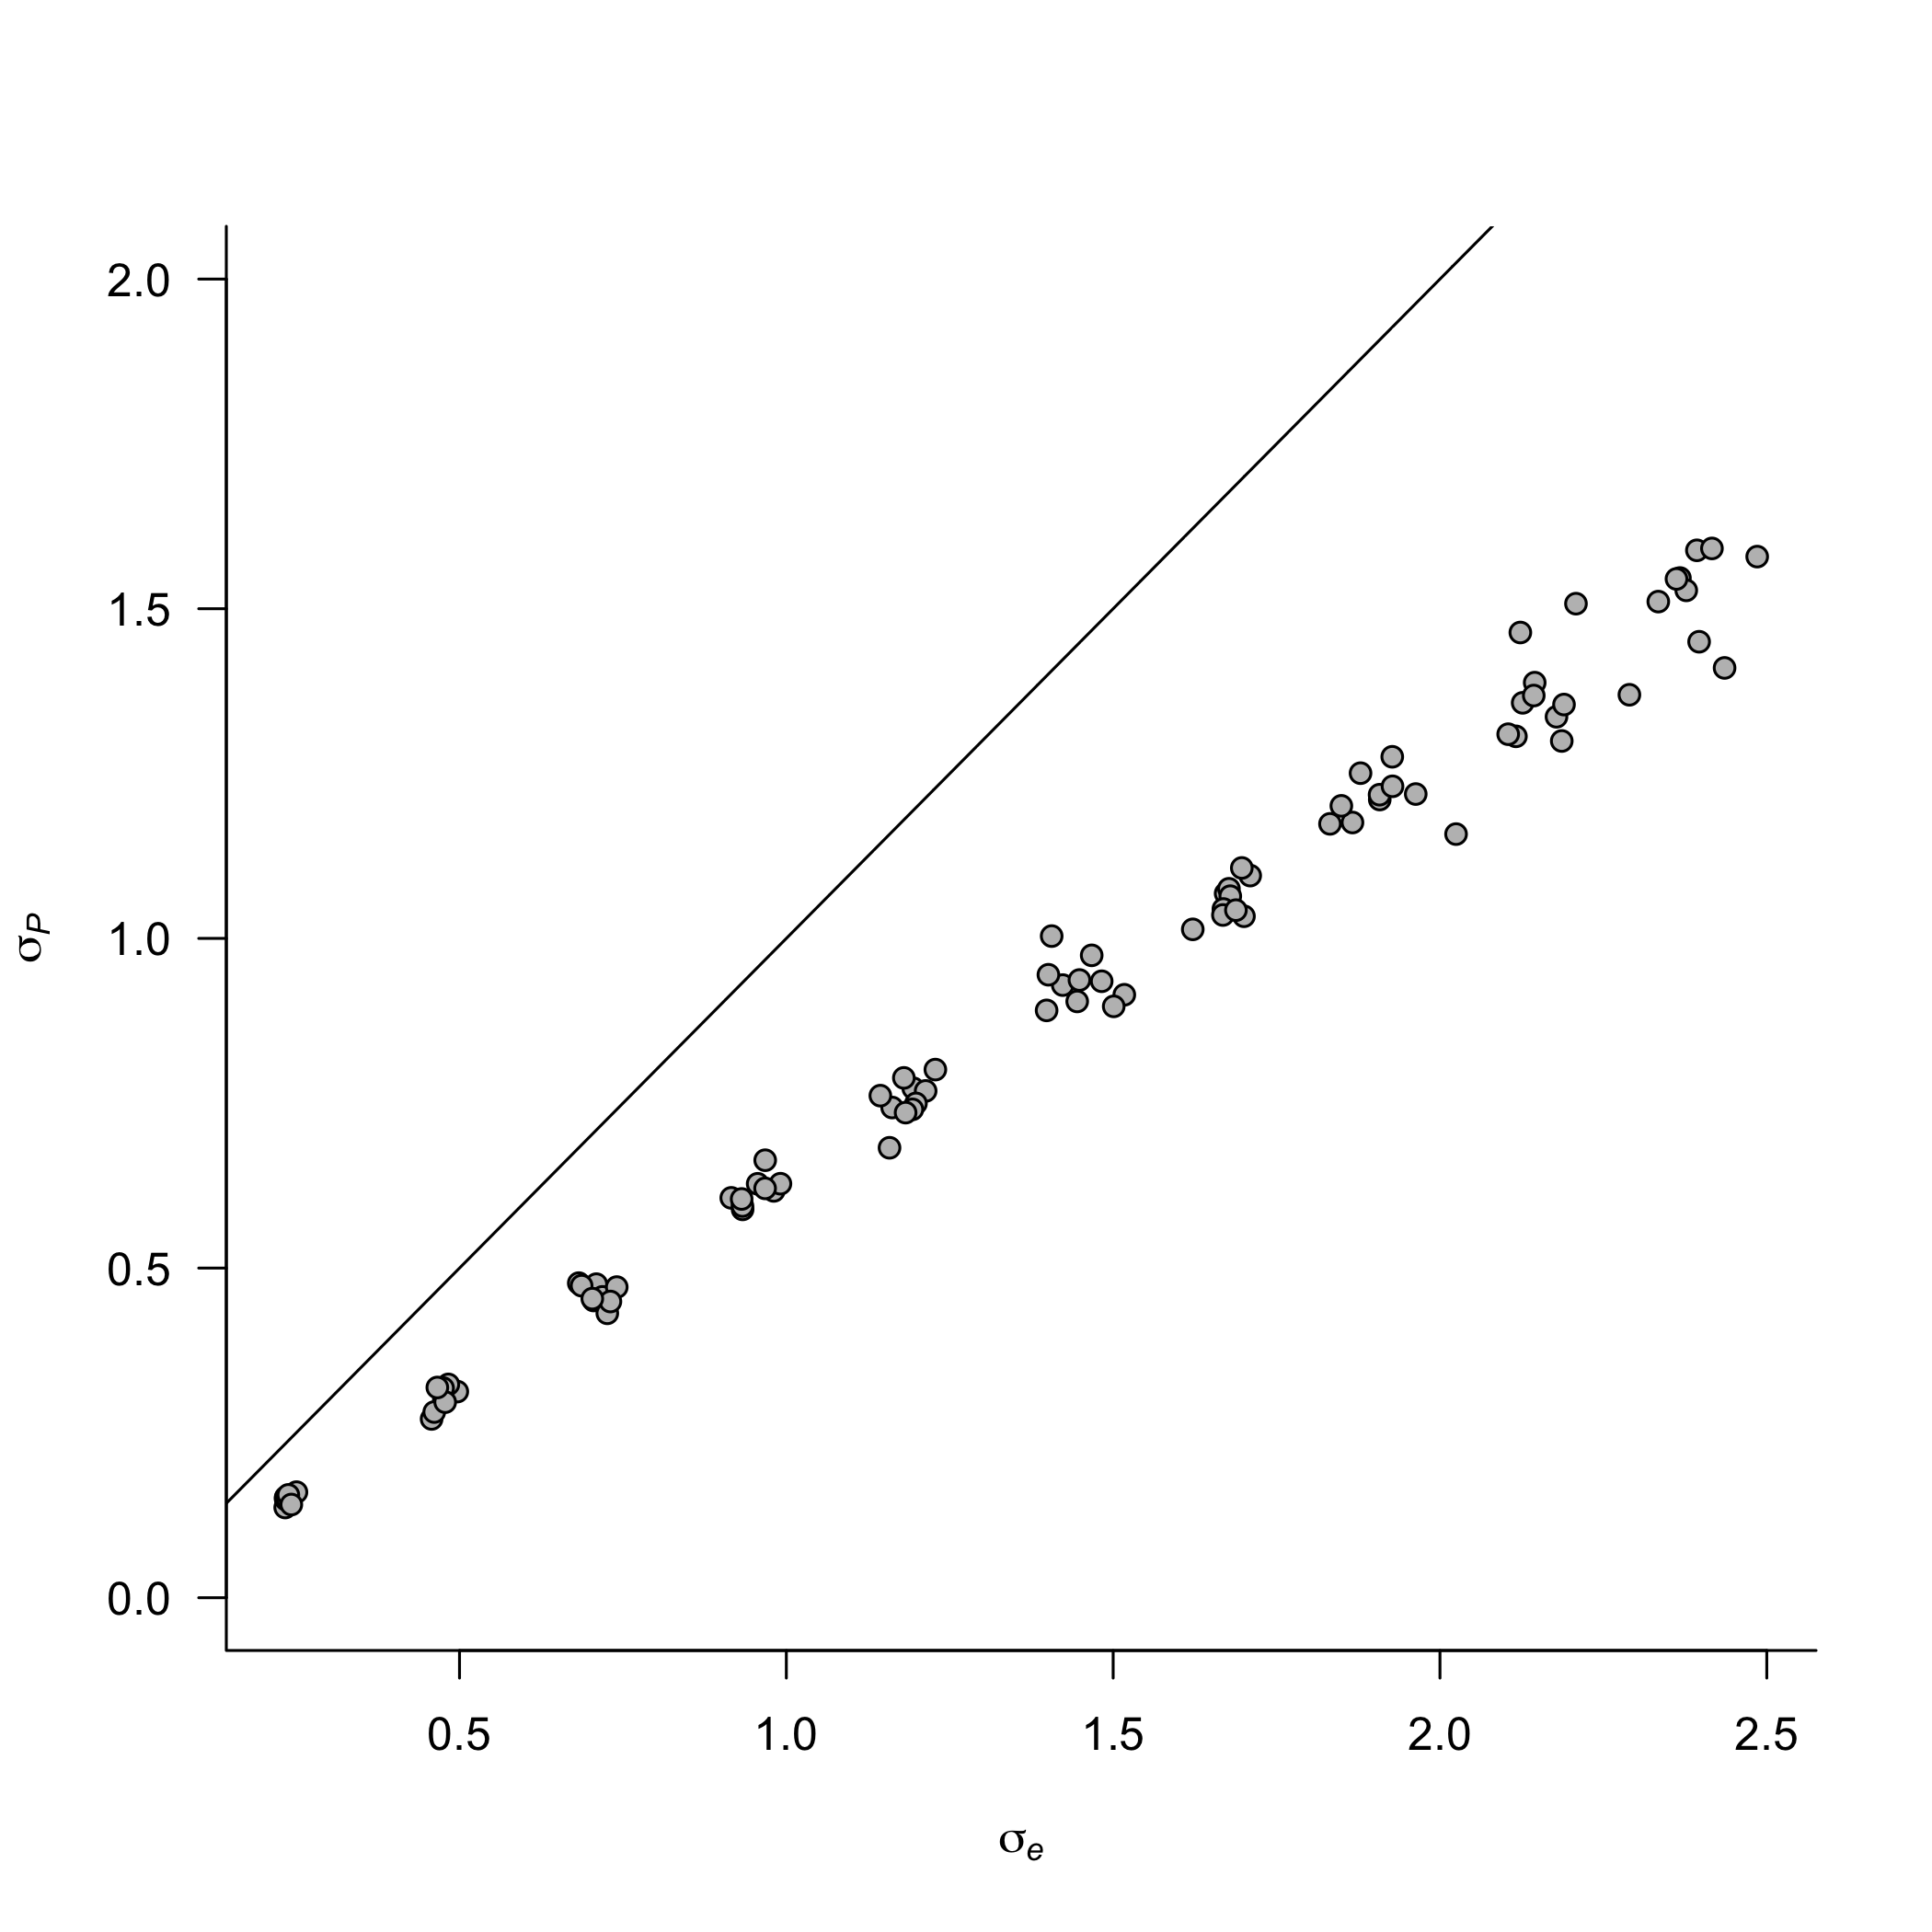
\includegraphics[width=\textwidth]{figs/gauss-rate-estimates}
\caption{Migration rate estimates for a Gaussian dispersal kernel. Each point
represents a single simulation generated under Gaussian dispersal with effective
migration rate given on the x-axis and a parsimonious genome-wide estimate of that
rate on the y-axis. The inset line shows a 1:1 relationship.
}
\label{fig:gauss-rate-estimates}
\end{figure}

\begin{figure}
\centering
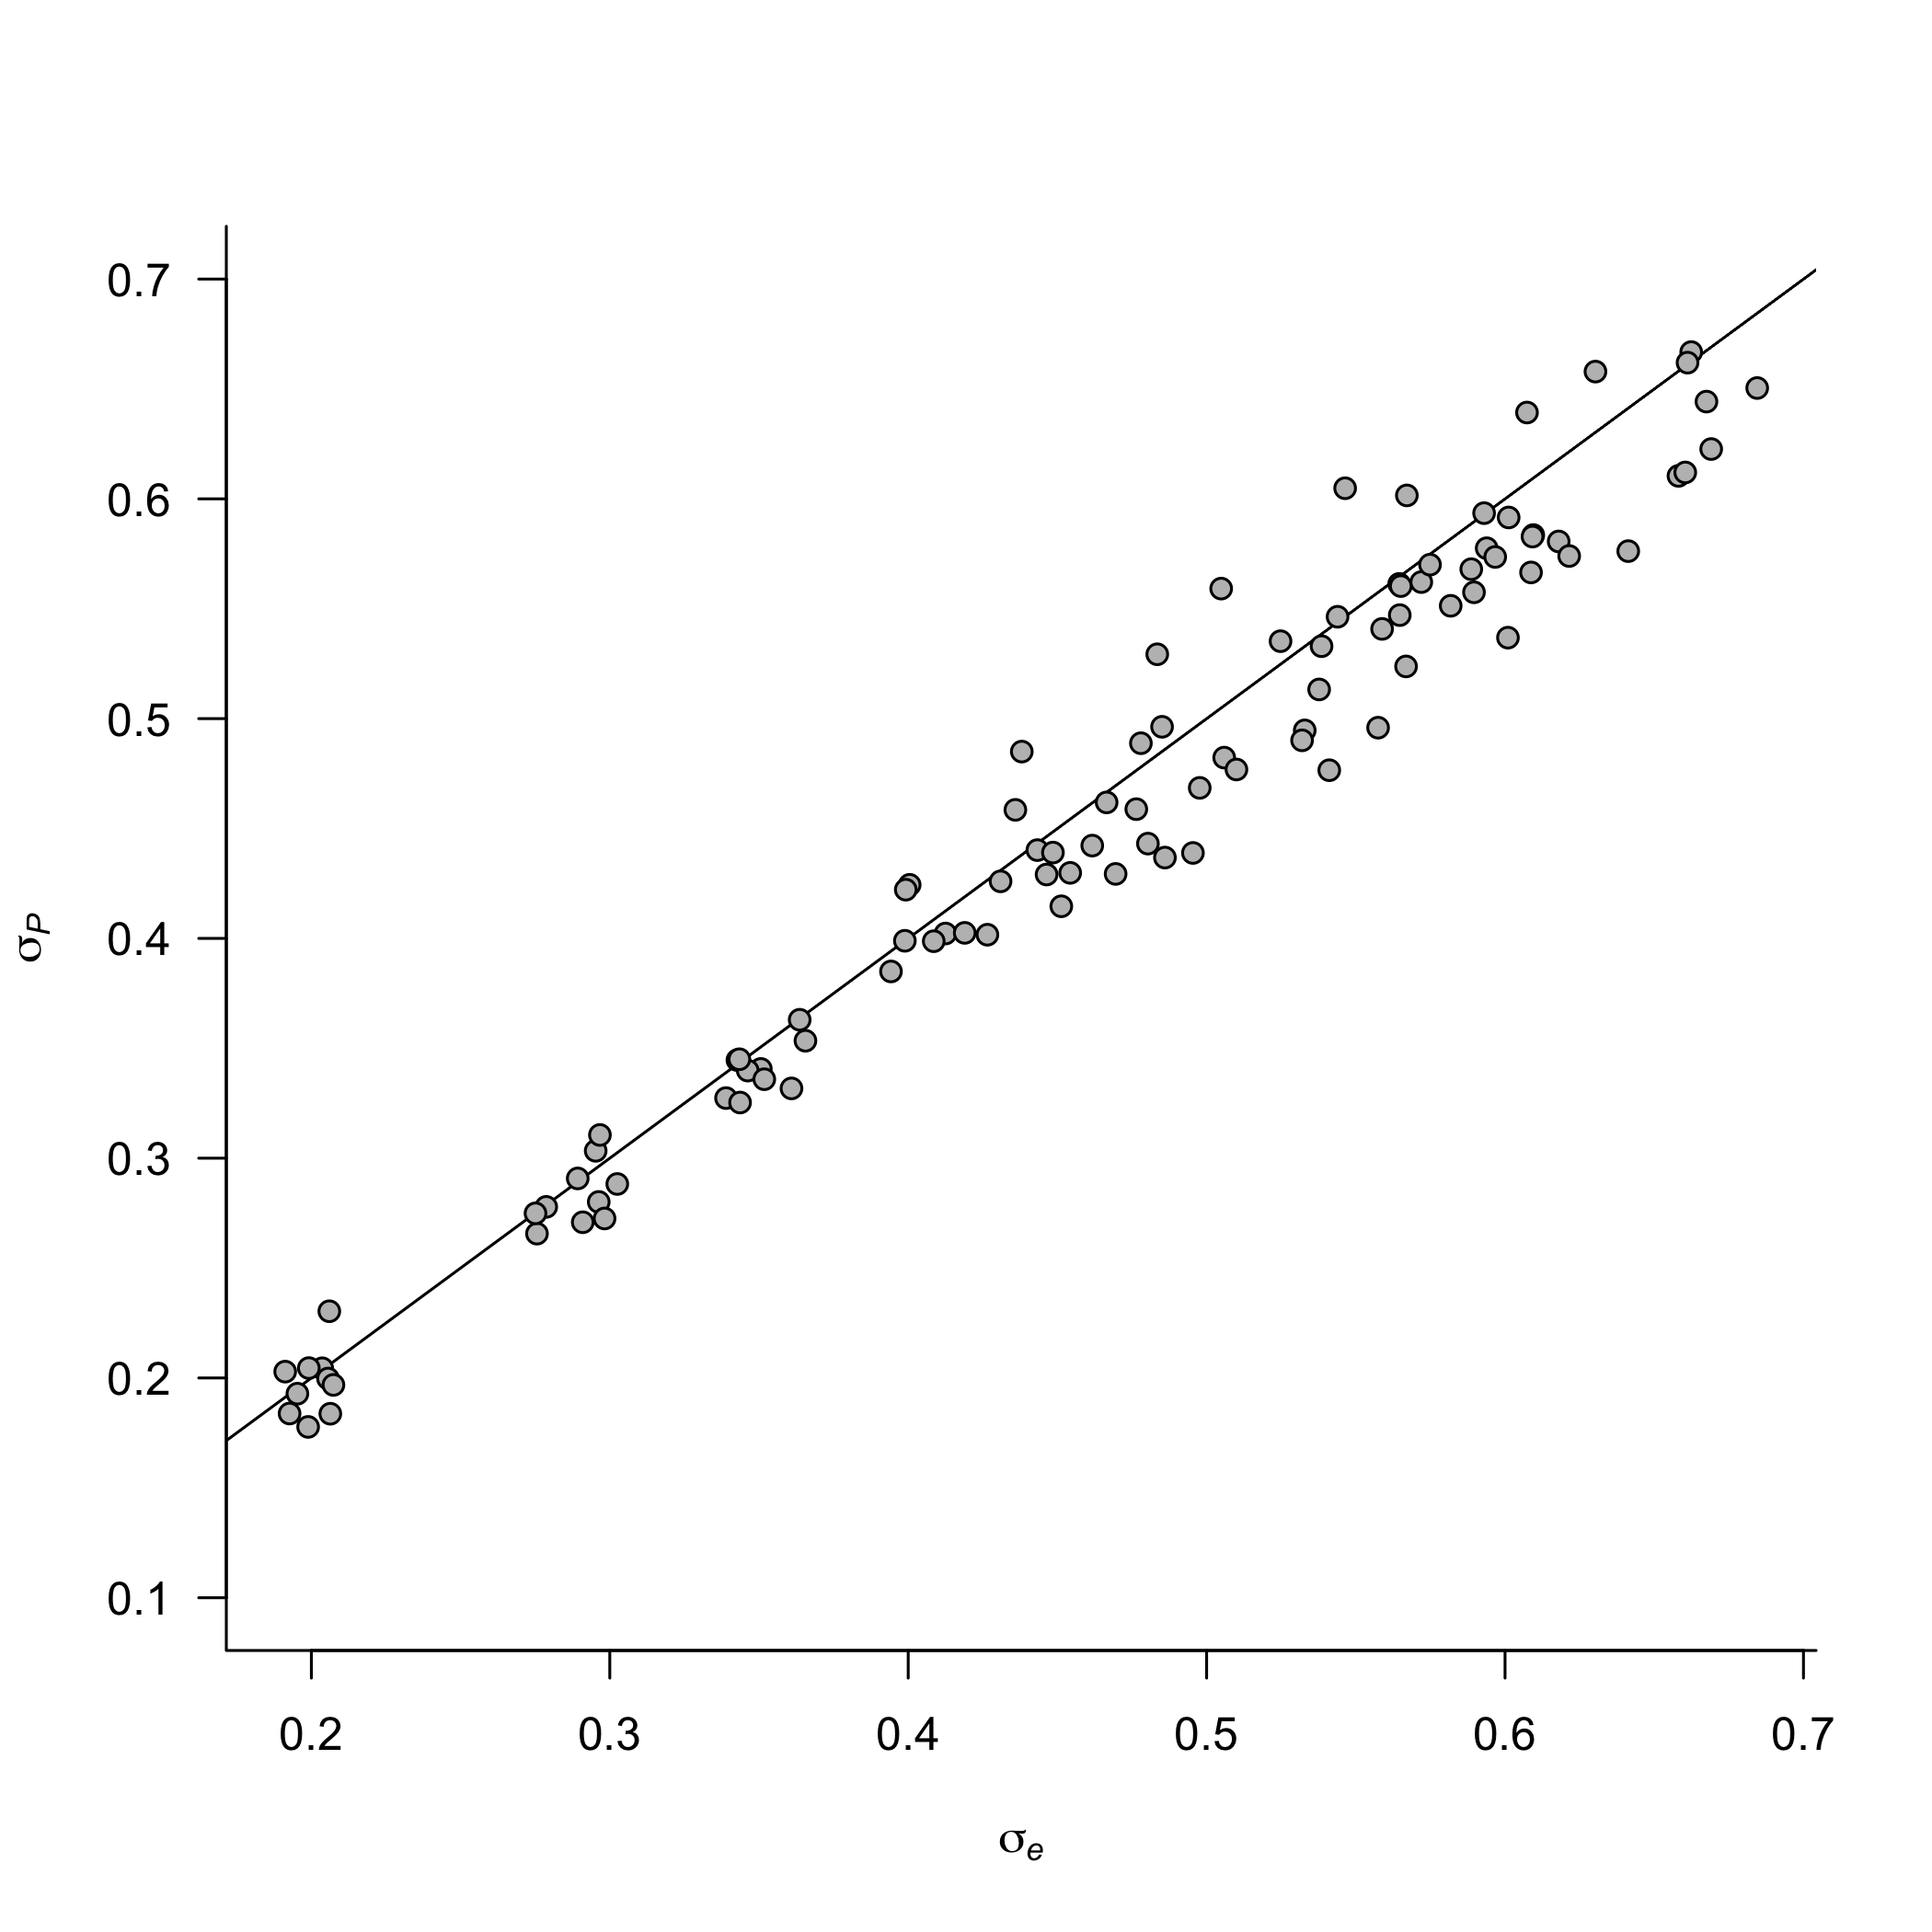
\includegraphics[width=\textwidth]{figs/lapl-rate-estimates}
\caption{Migration rate estimates for a Laplace dispersal kernel. Each point
represents a single simulation generated under Laplace dispersal with effective
migration rate given on the x-axis and a parsimonious genome-wide estimate of
that rate on the y-axis. The inset line shows a 1:1 relationship.
}
\label{fig:lapl-rate-estimates}
\end{figure}

\begin{figure}
\centering
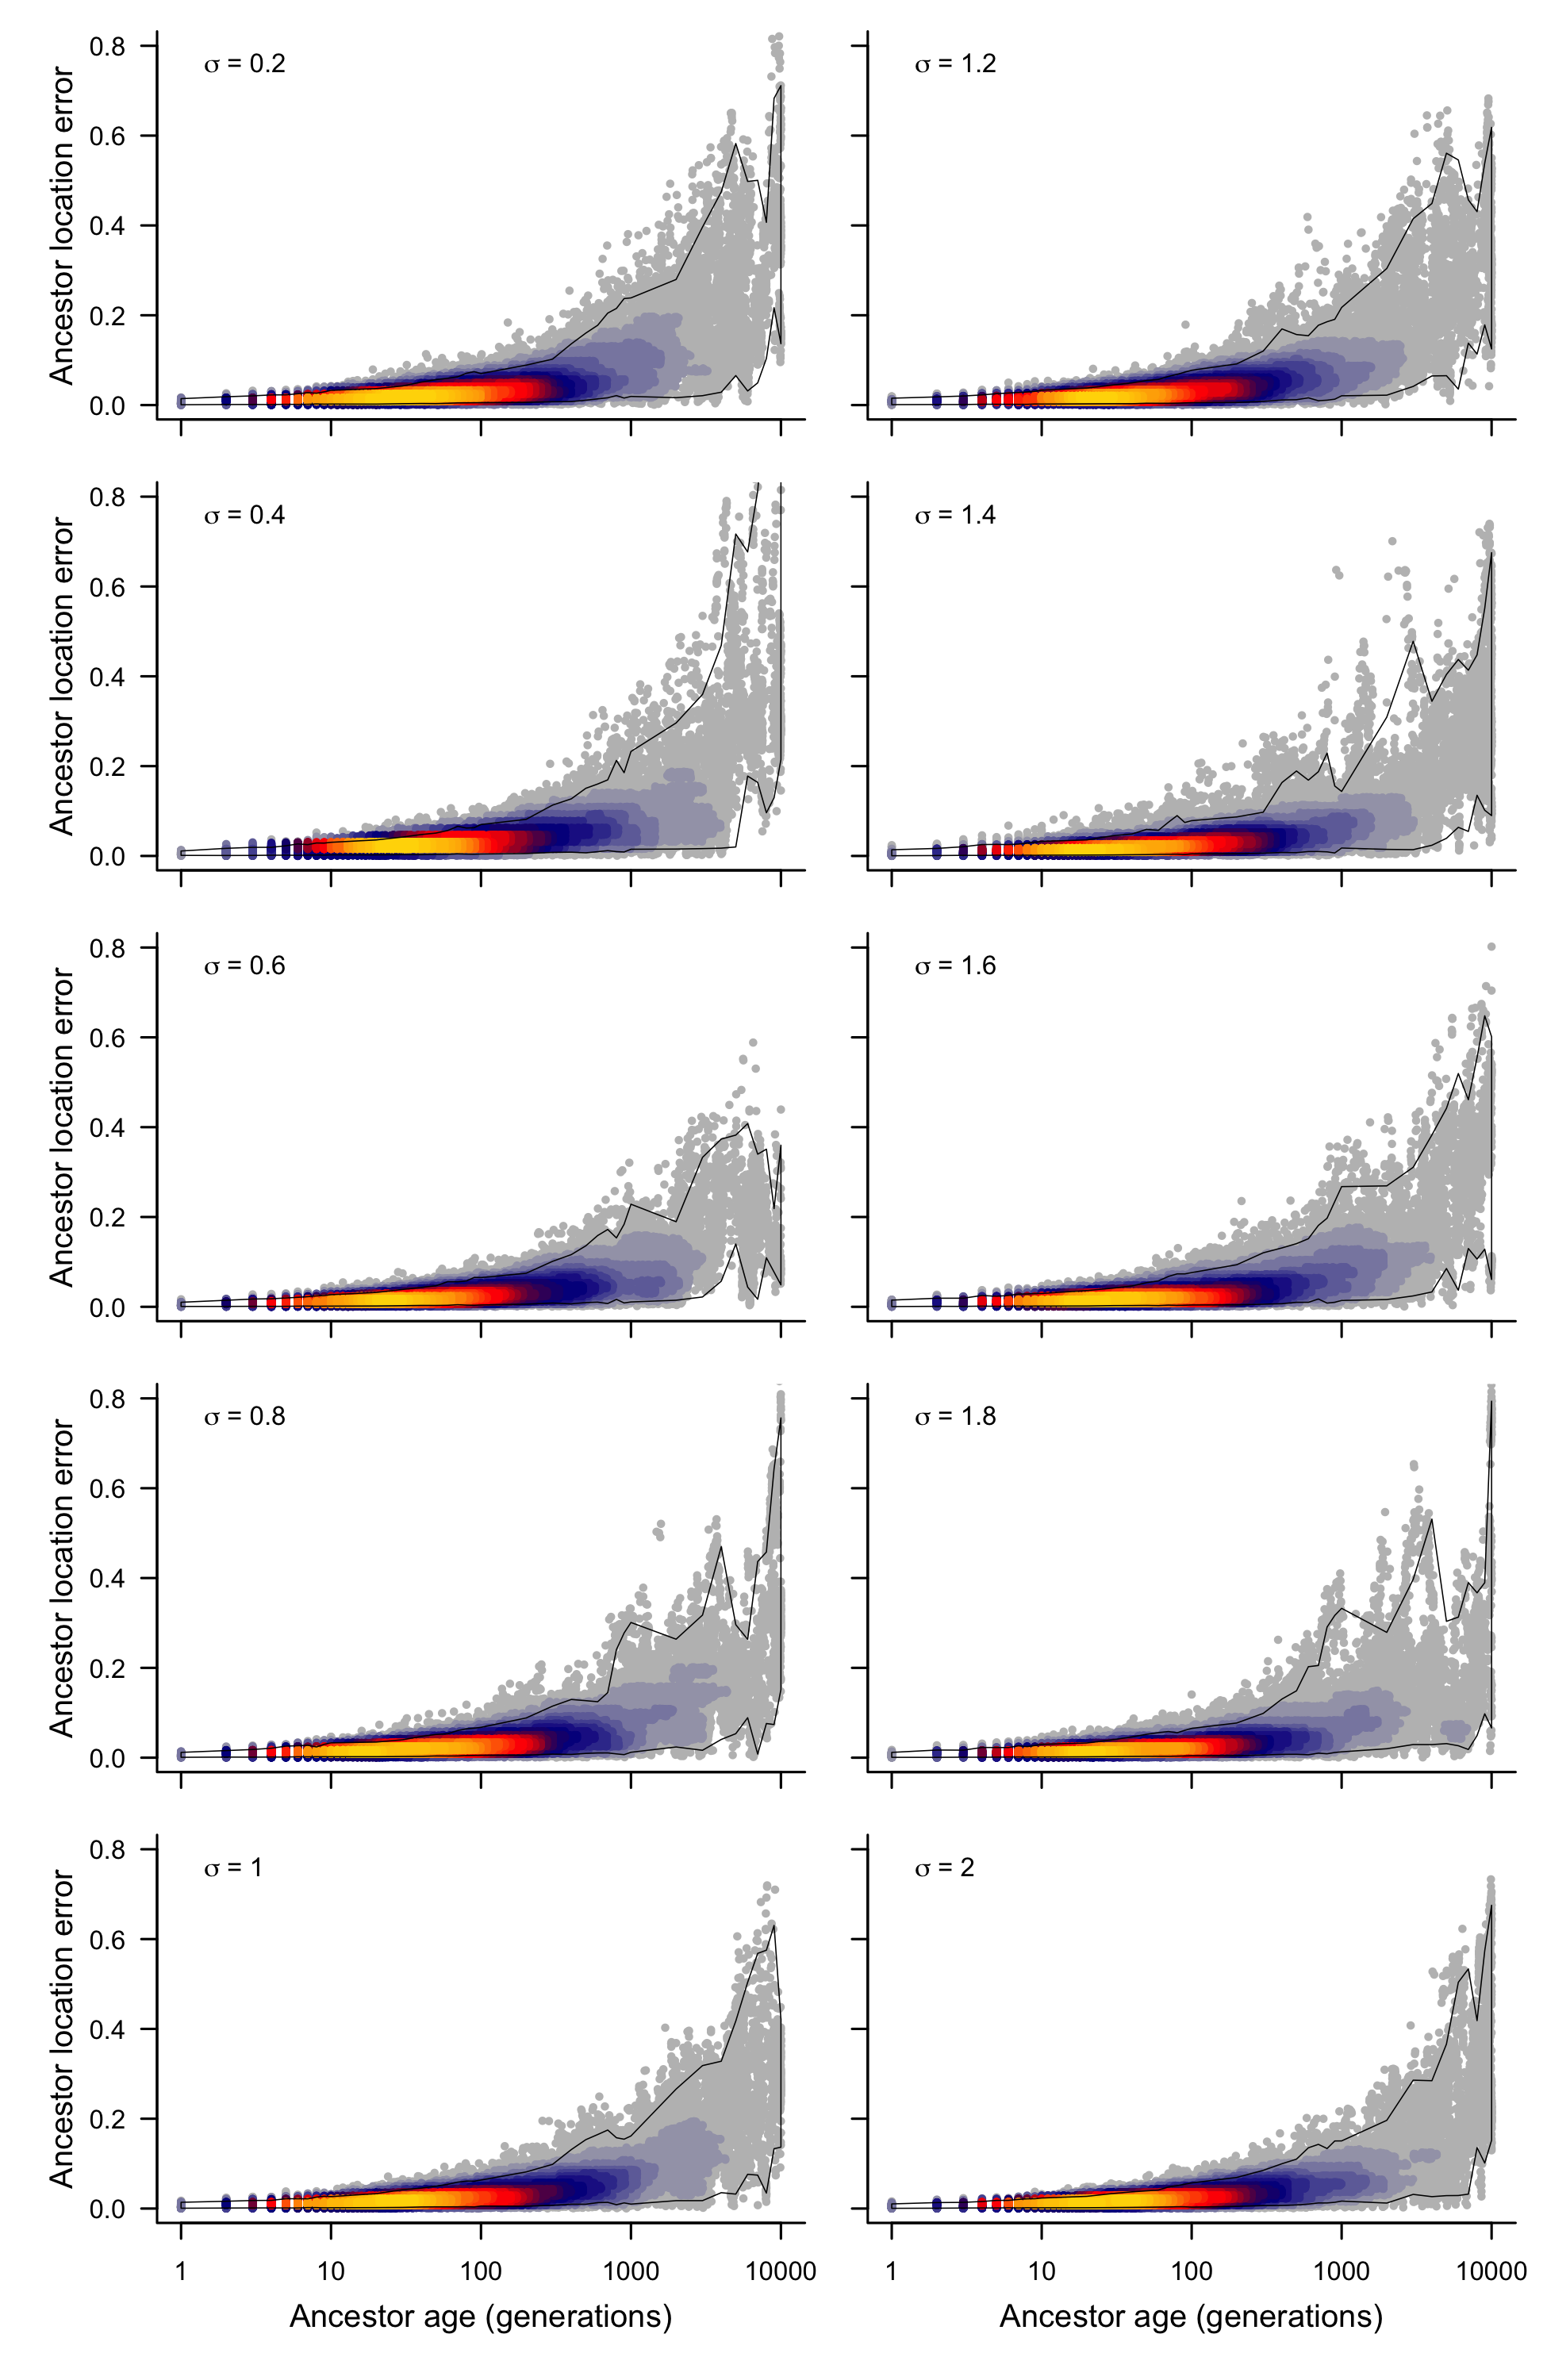
\includegraphics[width=0.75\textwidth]{figs/gauss-ancestor-estimates}
\caption{Ancestor location error for a Gaussian dispersal kernel. Each point
represents a single genetic ancestor. Ancestor location error is measured as
the distance between the estimated and the true location divided by the greatest
distance separating any pair of samples. Warm colors signify a greater density
of points. The envelope outlined in black encompasses 95\% of points.
}
\label{fig:gauss-ancestor-estimates}
\end{figure}

\begin{figure}
\centering
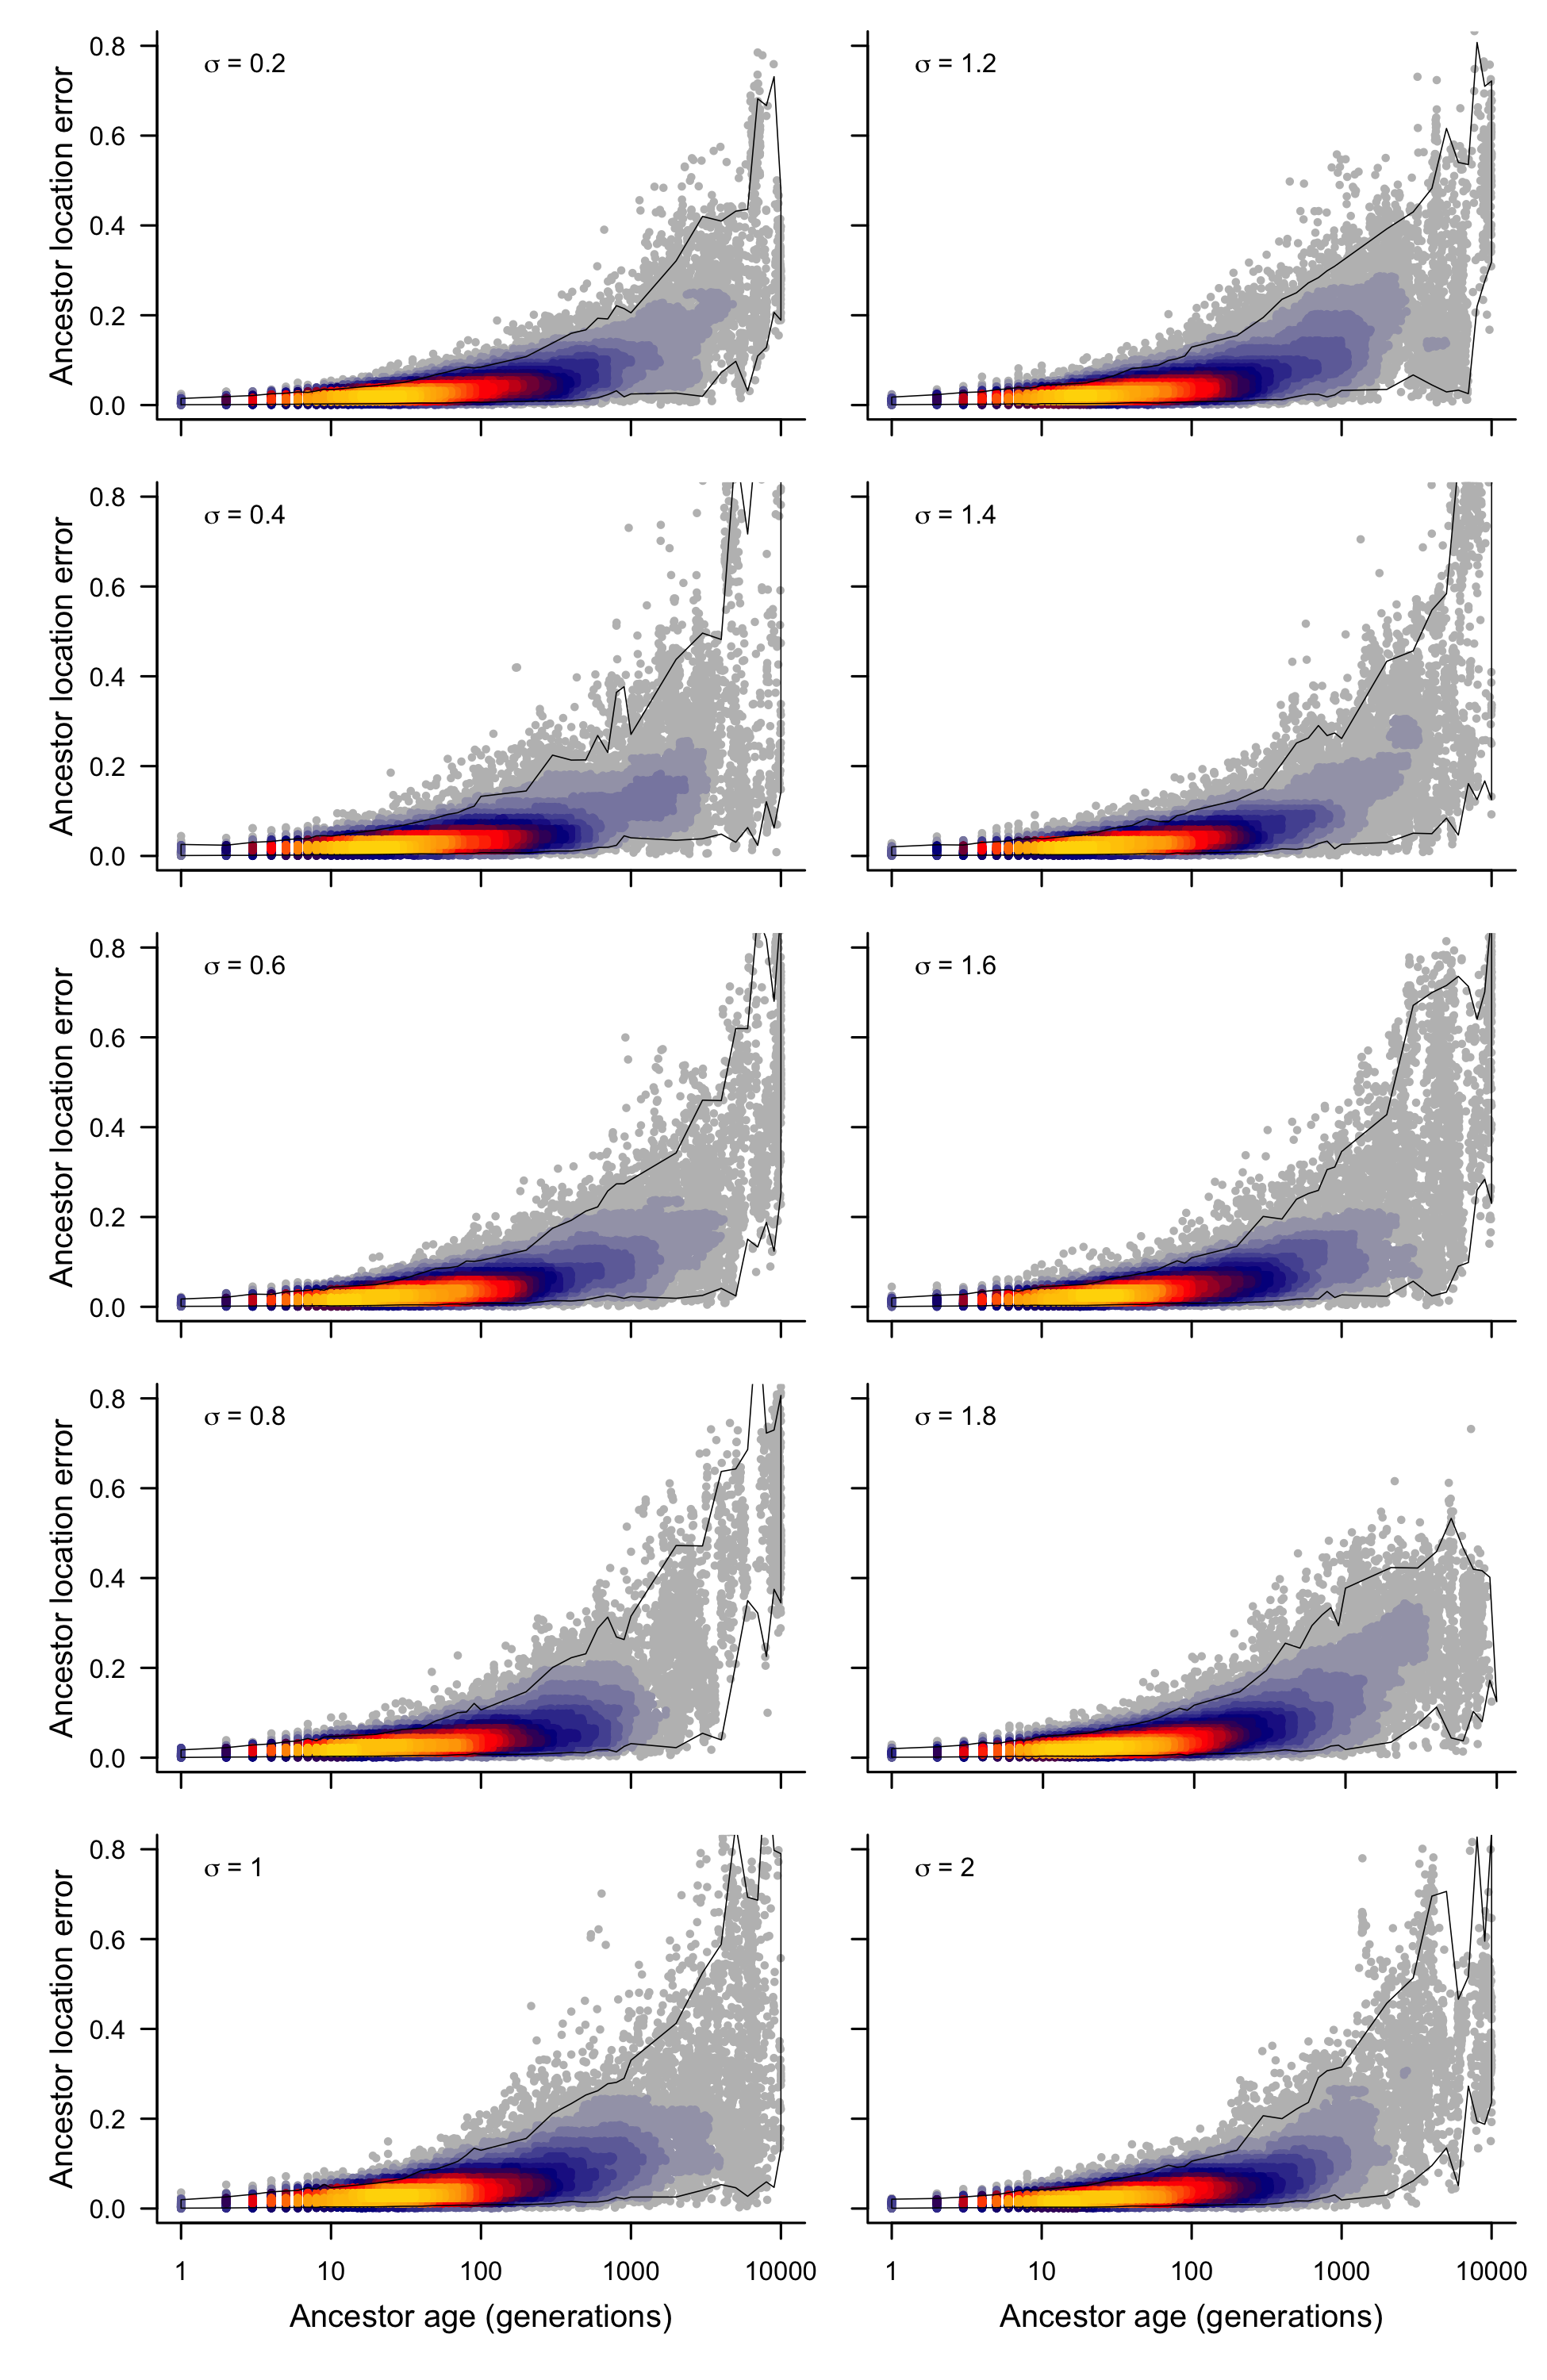
\includegraphics[width=0.75\textwidth]{figs/lapl-ancestor-estimates}
\caption{Ancestor location error for a Laplace dispersal kernel. Each point
represents a single genetic ancestor. Ancestor location error is measured as
the distance between the estimated and the true location divided by the greatest
distance separating any pair of samples. Warm colors signify a greater density
of points. The envelope outlined in black encompasses 95\% of points.
}
\label{fig:lapl-ancestor-estimates}
\end{figure}

\begin{figure}
\centering
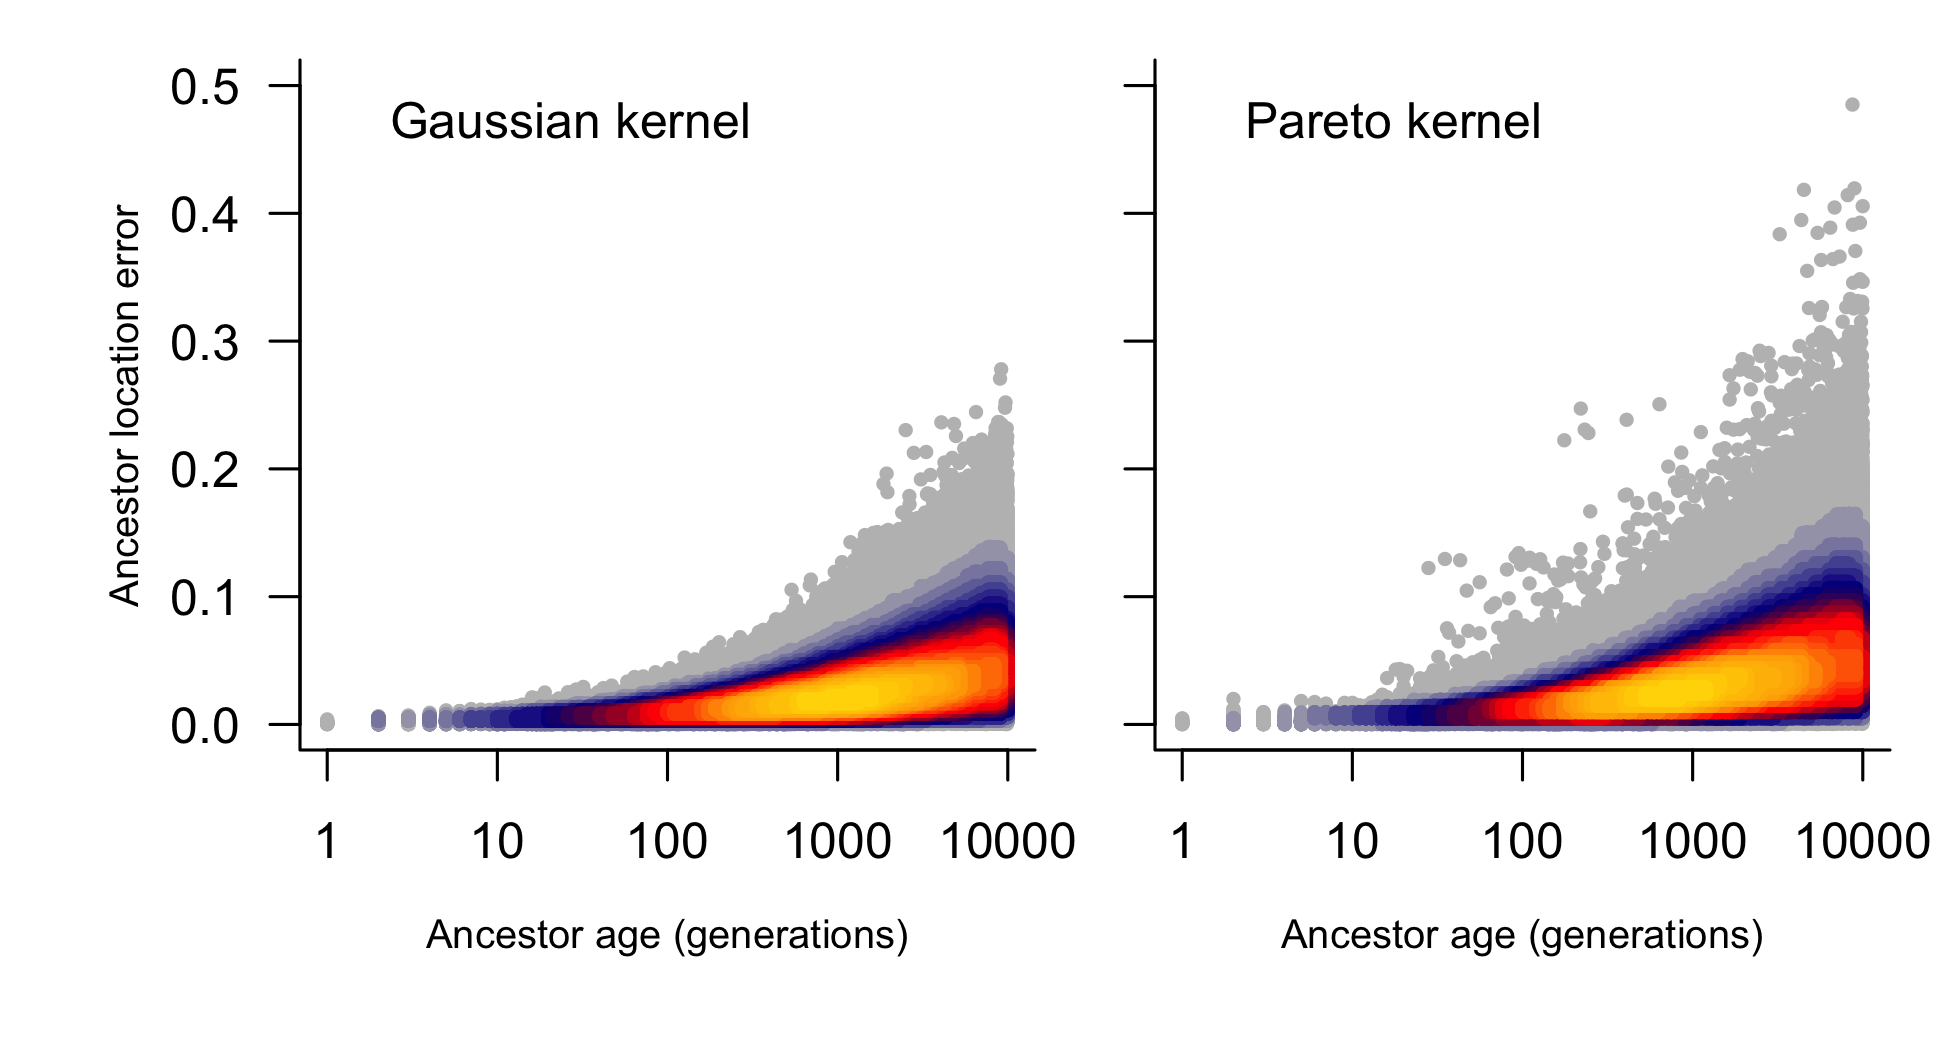
\includegraphics[width=\textwidth]{figs/heterogeneous-ancestor-estimates}
\caption{Ancestor location error for a Gaussian dispersal kernel (left) or a
Pareto dispersal kernel (right) on simulated landscapes with spatially varying
carrying capacity. Each point represents a single genetic ancestor. Ancestor
location error is measured as the distance between the estimated and the true 
location divided by the greatest distance separating any pair of samples. 
Warm colors signify a greater density of points. The envelope outlined in black 
encompasses 95\% of points.
}
\label{fig:heterogeneous-ancestor-estimates}
\end{figure}

\begin{figure}
\centering
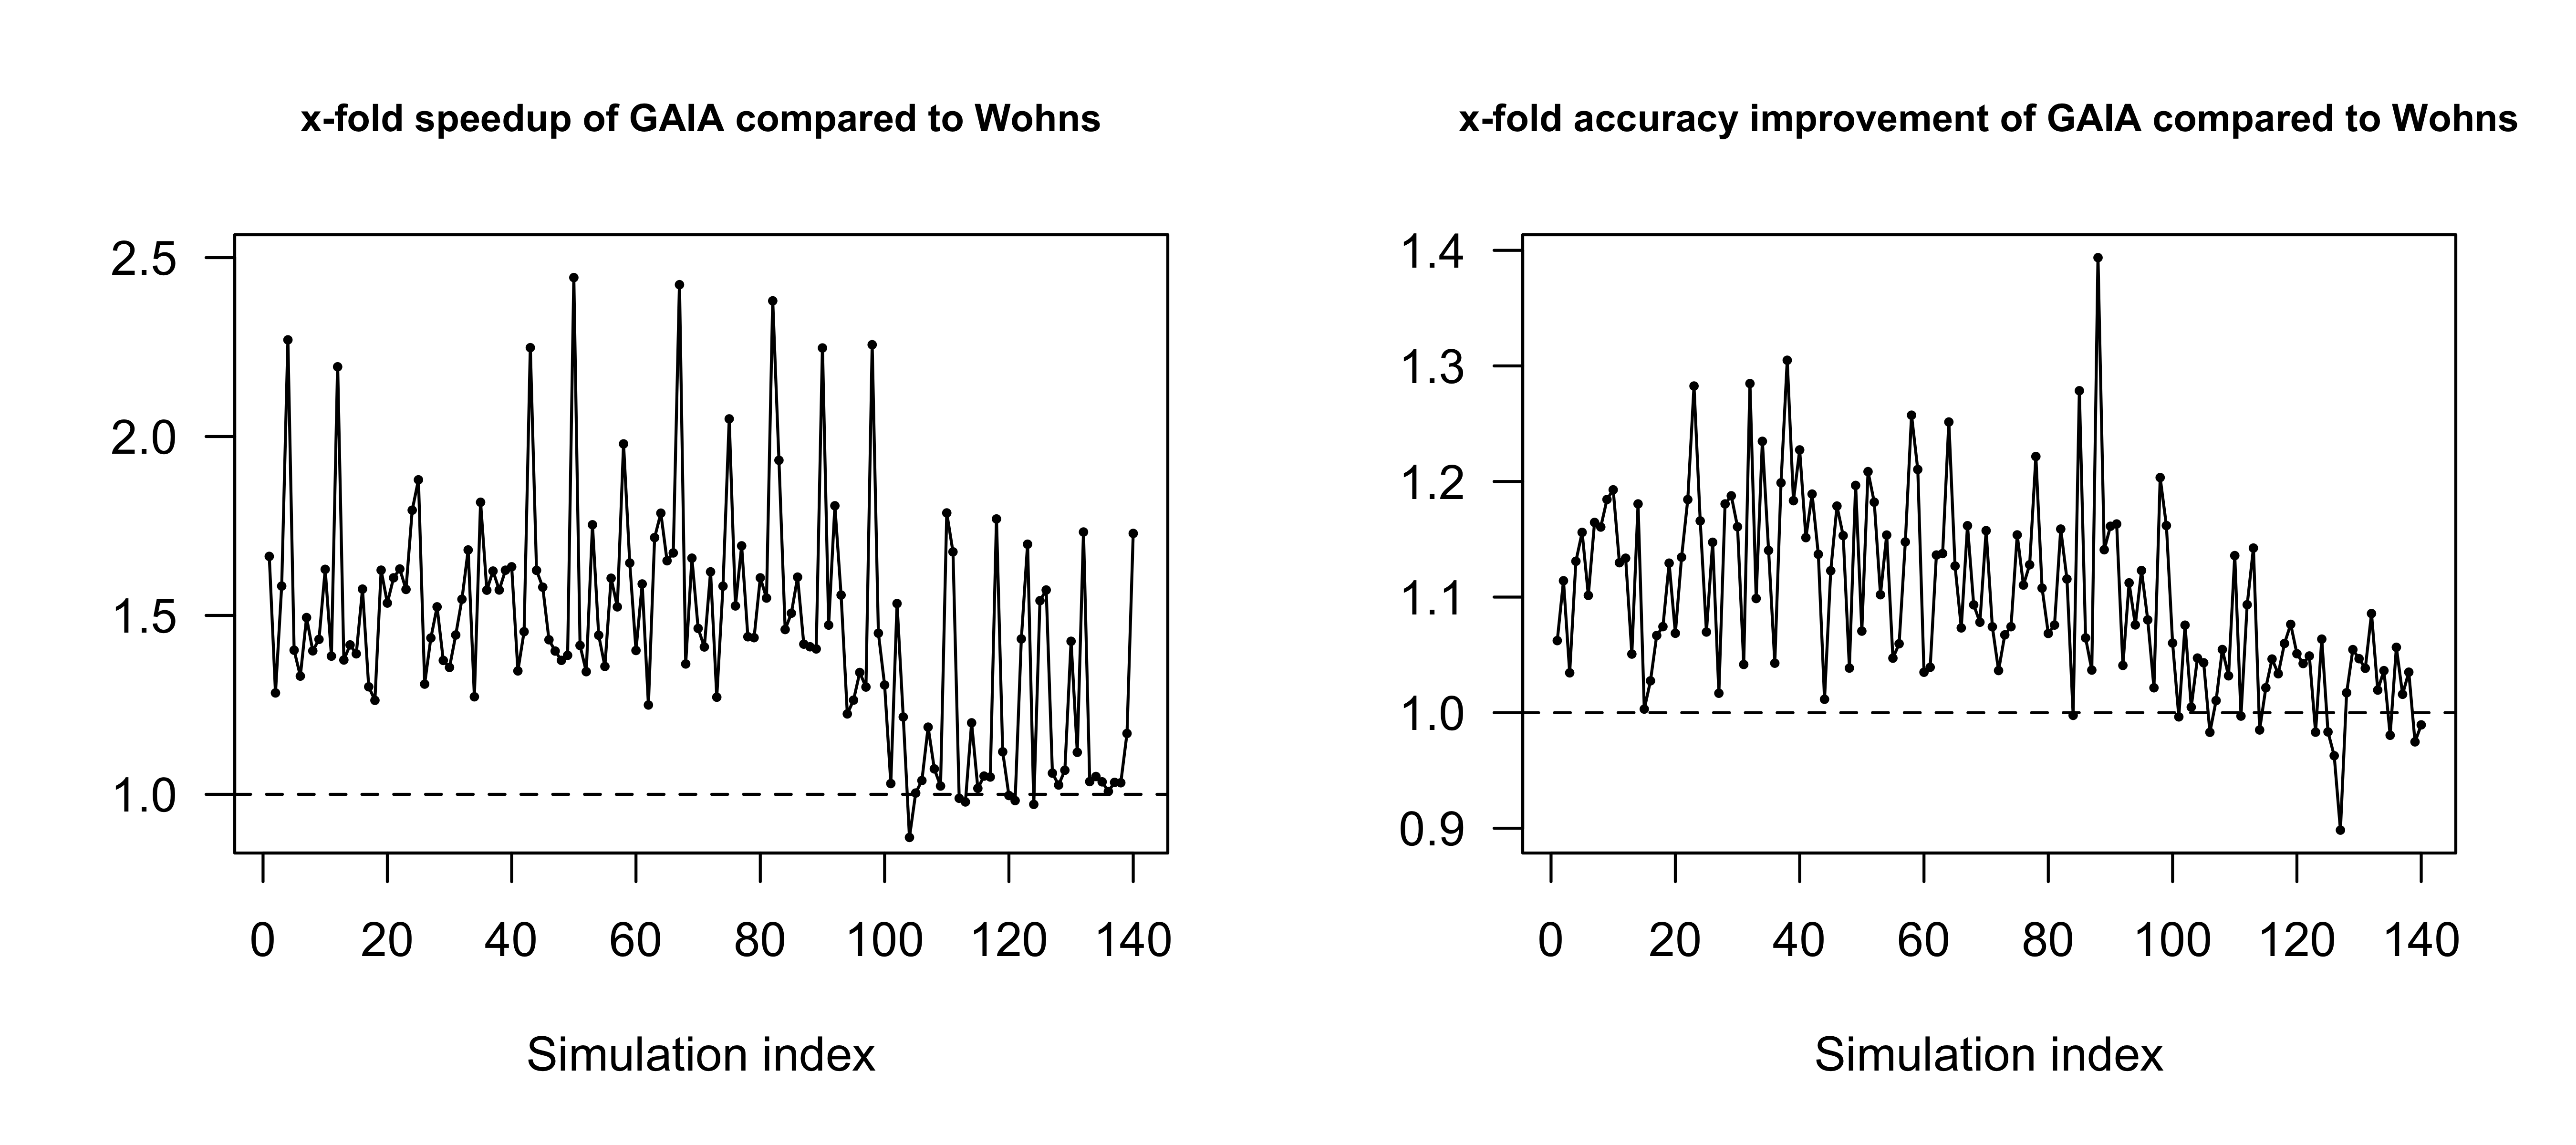
\includegraphics[width=\textwidth]{figs/gaia-wohns-compare}
\caption{Comparison of ancestor location inference accuracy (right) and computational
timings (left) between \textsc{gaia} and the non-parametric method of 
~\cite{Wohns_etal_2022}. Each point represents a single SLiM simulation on a
continuous landscape. Values greater than 1 indicate greater accuracy and speed
of \texttt{gaia} relative to the alternative method. Indices 1-100 correspond to Gaussian dispersal on a
uniform landscape; 101-120, to Gaussian dispersal on a heterogeneous landscape; 
121-140, to Pareto dispersal on a heterogeneous landscape. Timings were conducted
on a 2023 Macbook Pro with 18Gb of RAM and an Apple M3 Pro chip.
}
\label{fig:gaia-wohns-compare}
\end{figure}

\begin{figure}
\centering
{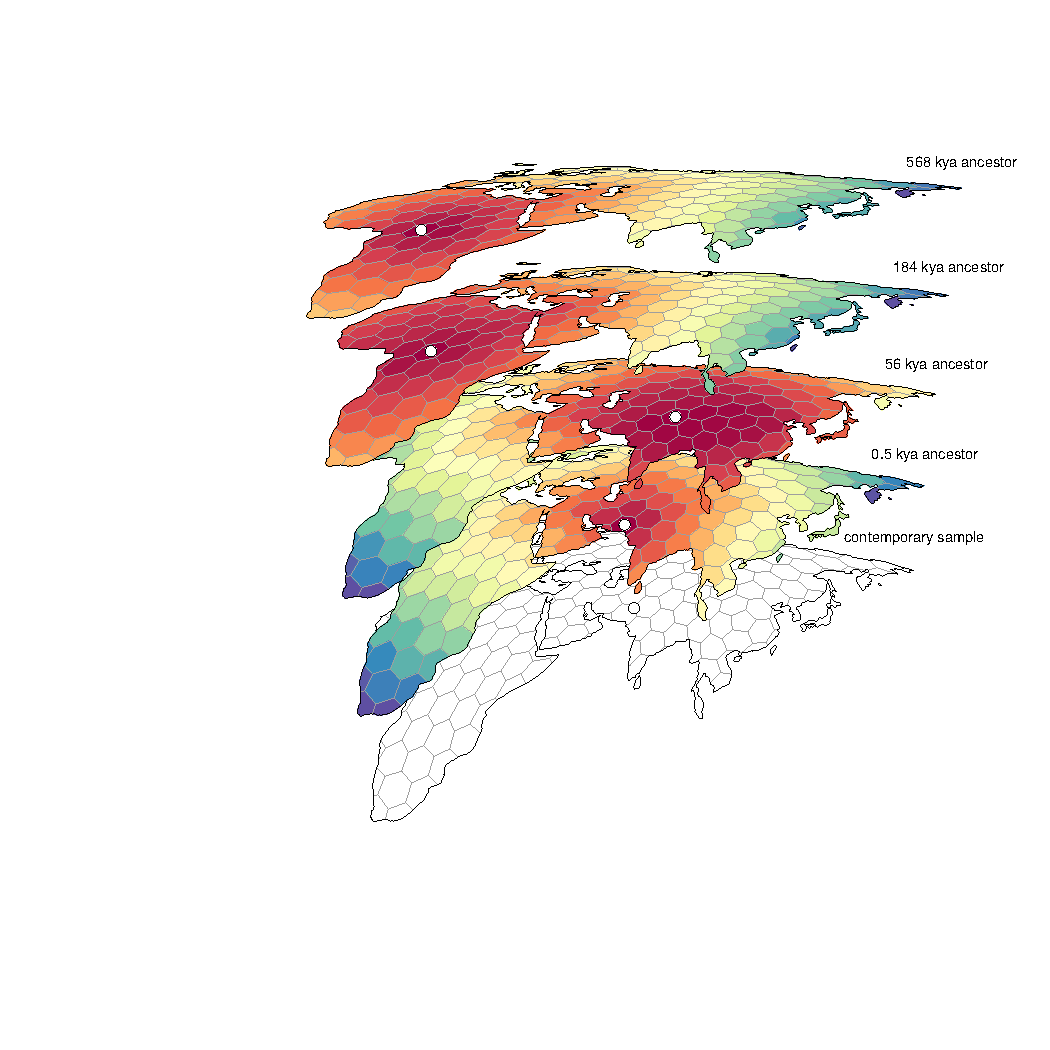
\includegraphics[width=\textwidth]{figs/uncertainty.pdf}}

\caption{An example set of geographically referenced genetic ancestors of a
contemporary sample from Asia. Colored grid cells denote the migration costs
calculated by \textsc{gaia} (warmer colors denote lower costs) and each ancestor 
(denoted by a white point) is positioned within the minimum cost grid cell. For 
most ancestors there are many near-optimal locations that are ignored by our
summary methods, which should therefore be viewed as summarizing major trends
rather than as precise statements on where ancestors lived and how they moved.}
\label{fig:uncertainty}

\end{figure}

\begin{figure}
\centering
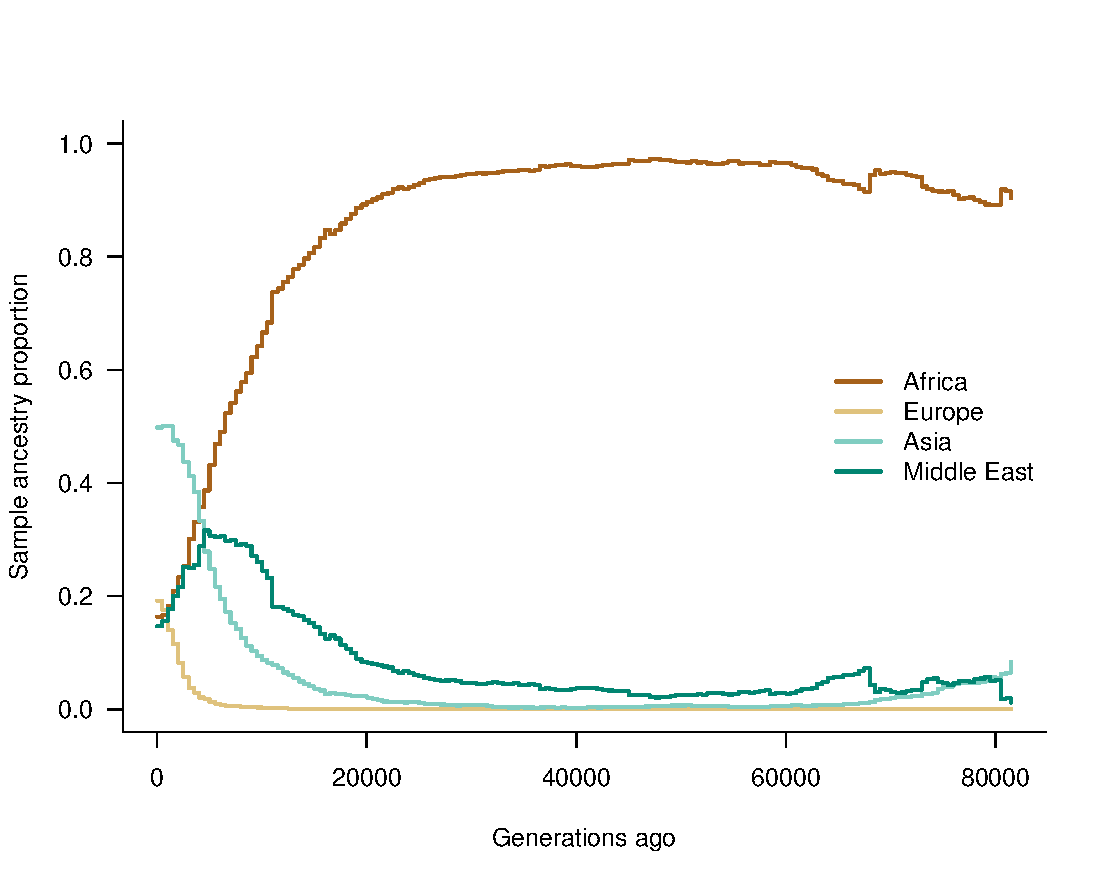
\includegraphics[width=\textwidth]{figs/overall-ancestry}
\caption{Inferred spatiotemporal ancestry coefficients computed from the
entire sample at equally spaced 500 generation intervals back through time.
Lines depict the fraction of genomic positions in the sample that trace 
ancestry to the different geographic regions at different points in time. The
decline in genetic ancestry found in Africa in the ancient past likely reflects
attenuation of phylogenetic signal at deep time scales causing \textsc{gaia}
to misplace some genetic ancestors.
}
\label{fig:overall-ancestry}
\end{figure}

\begin{figure}
\centering
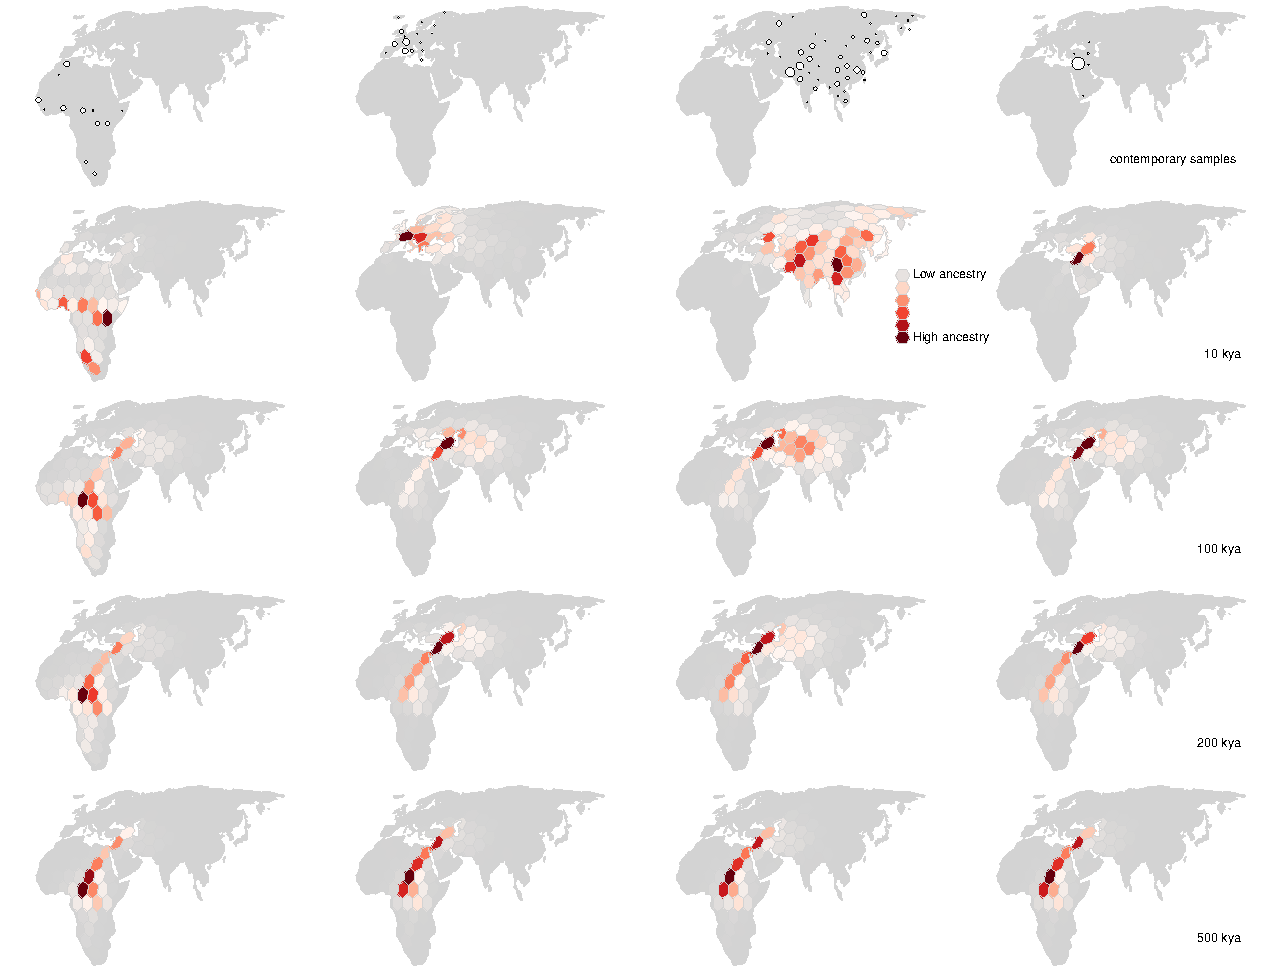
\includegraphics[width=\textwidth]{figs/ancestry-thru-time-subset-avg}
\caption{Inferred spatiotemporal ancestry coefficients through time averaged
from 100 random subsets of the data. The fraction of genomic positions in each 
geographic subset of samples (top row) that trace ancestry to different
geographic regions at different times in the past is represented by shades of 
red, with darker shading indicating greater ancestry (=a larger fraction). 
Point size is proportional to the number of sampled genomes from each 
locality in the full dataset. Subsets of the data were taken by randomly 
downsampling localities so that each was represented by a single individual.
Variation about these averages is shown in Fig \ref{fig:ancestry-subset-sdev}.
}
\label{fig:ancestry-subset-avg}
\end{figure}

\begin{figure}
\centering
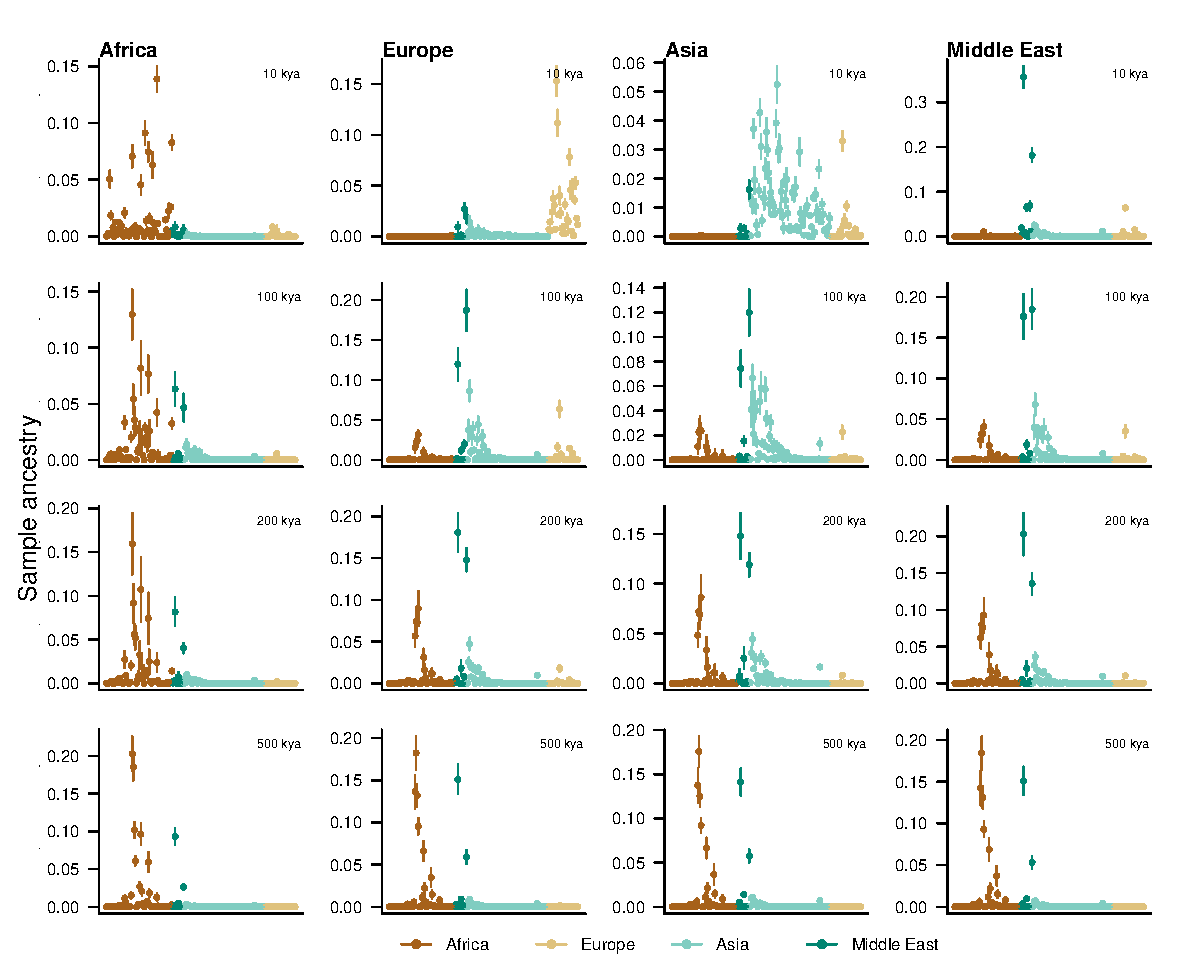
\includegraphics[width=\textwidth]{figs/ancestry-thru-time-sdev}
\caption{Variance in spatiotemporal ancestry coefficients over 100 random
subsets of the data. Columns record the average spatial temporal ancestry
coefficients at 4 different time slices for samples in the 4 geographic
regions. Each point corresponds to a hexcell and is colored by the
major geographic region in which it is situated. The mean spatiotemporal
ancestry coefficient for each cell is bracketed by one standard deviation.
}
\label{fig:ancestry-subset-sdev}
\end{figure}

\begin{figure}
\centering
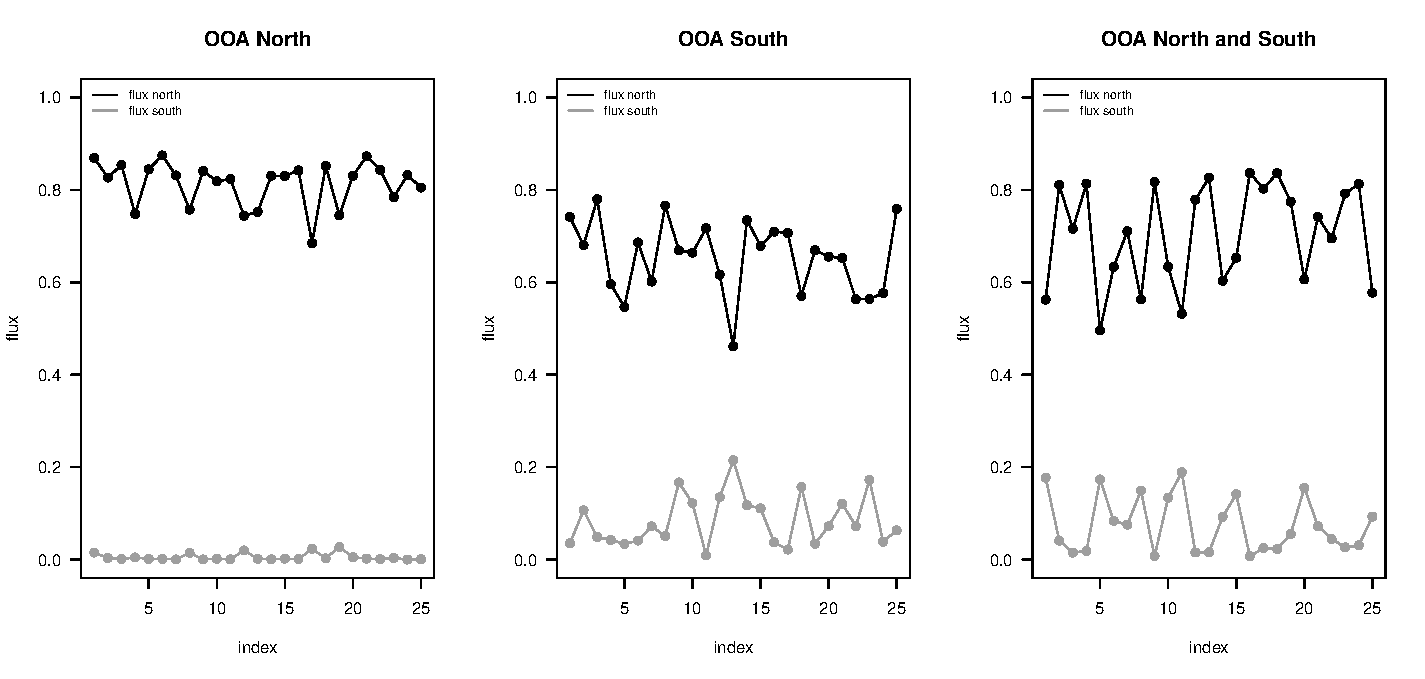
\includegraphics[width=\textwidth]{figs/ooa-sim-flux}
\caption{Estimated flux in spatiotemporal ancestry coefficients out of Africa
through northern and southern routes under simulation scenarios with different
available dispersal routes. Each point represents a single simulation. Simulations
in the left panel could only disperse out of Africa following a northern
route; simulations in the center panel could only disperse following a
southerly route; simulations in the right panel could disperse following either
route. All simulations were initiated from a single subpopulation in east
Africa. For all scenarios \textsc{gaia} estimates are biased through the
northern route.
}
\label{fig:ooa-sim-flux-bias}
\end{figure}

\begin{figure}
\centering
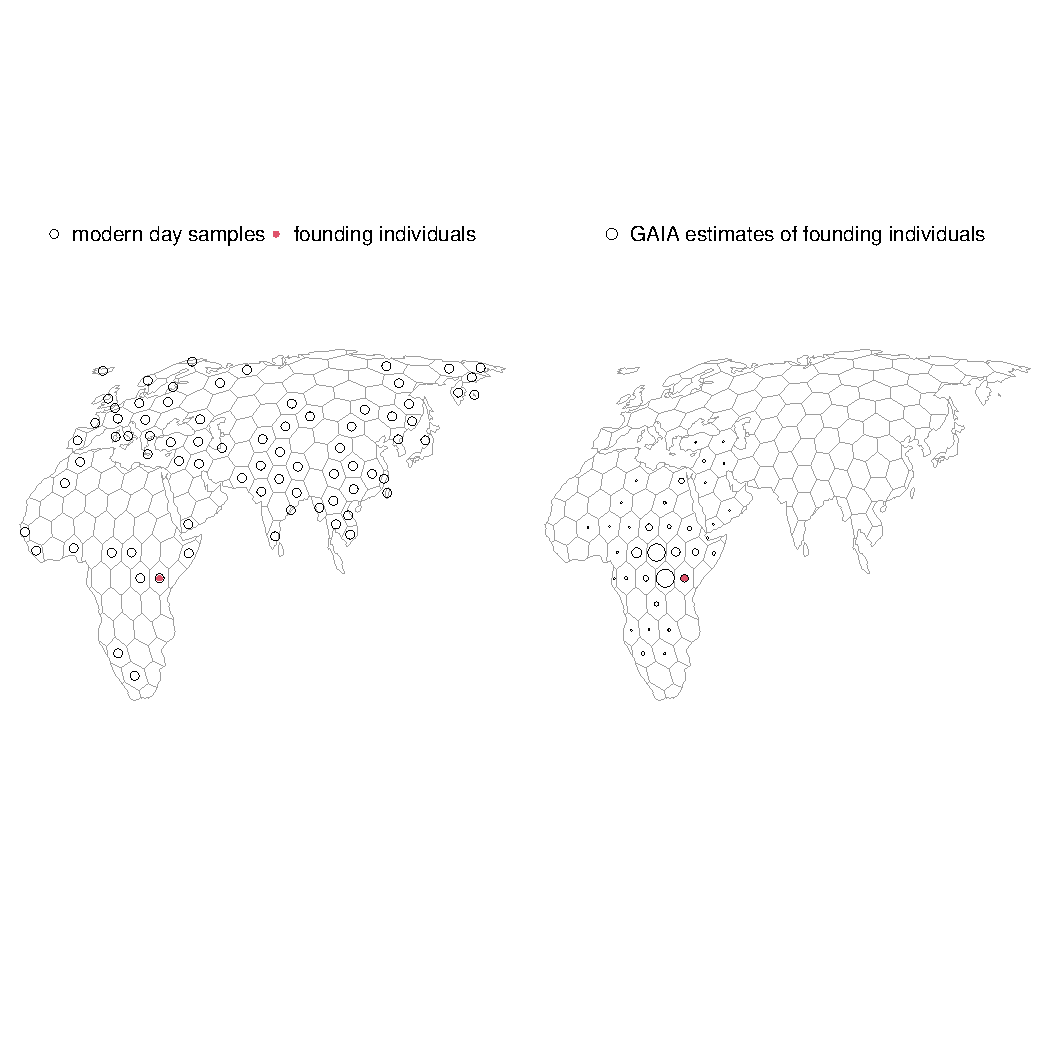
\includegraphics[width=\textwidth]{figs/ooa-sim-ancestor-estimates}
\caption{The left panel shows the distribution of a sample of modern-day individuals 
descended from a founding subpopulation in east Africa 20000 years ago. The 
right panel shows a frequency distribution of where founding individuals are 
estimated to have lived across replicate simulations. While \textsc{gaia} is
broadly correct in reconstructing ancestors in Africa, the estimates are pulled
away from the true location toward the centroid location of modern-day samples
from Africa. 
}
\label{fig:ooa-ancestor-estimate-bias}
\end{figure}

\begin{figure}
\centering
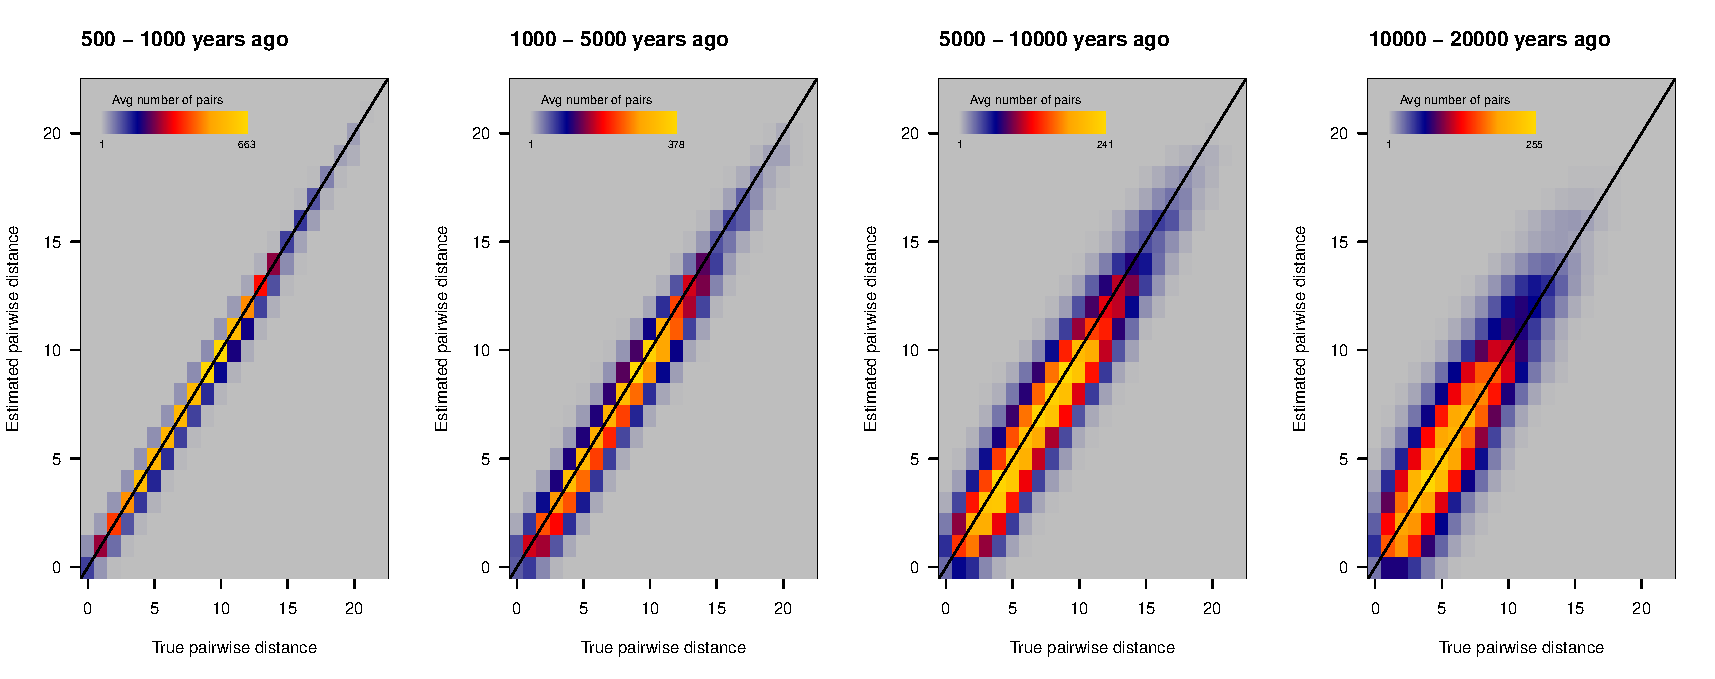
\includegraphics[width=\textwidth]{figs/ooa-pairwise-distances}
\caption{Relationship between true and estimated pairwise distances between
genetic ancestors of different age classes averaged over out-of-Africa 
simulation replicates. There is a slight tendency for \textsc{gaia} to place
ancestors closer together than they actually are, but the overall pairwise
distribution of ancestor-to-ancestor distances is recovered with high
accuracy in these simulations.
}
\label{fig:ooa-pairwise-distances}
\end{figure}

\begin{figure}
\centering
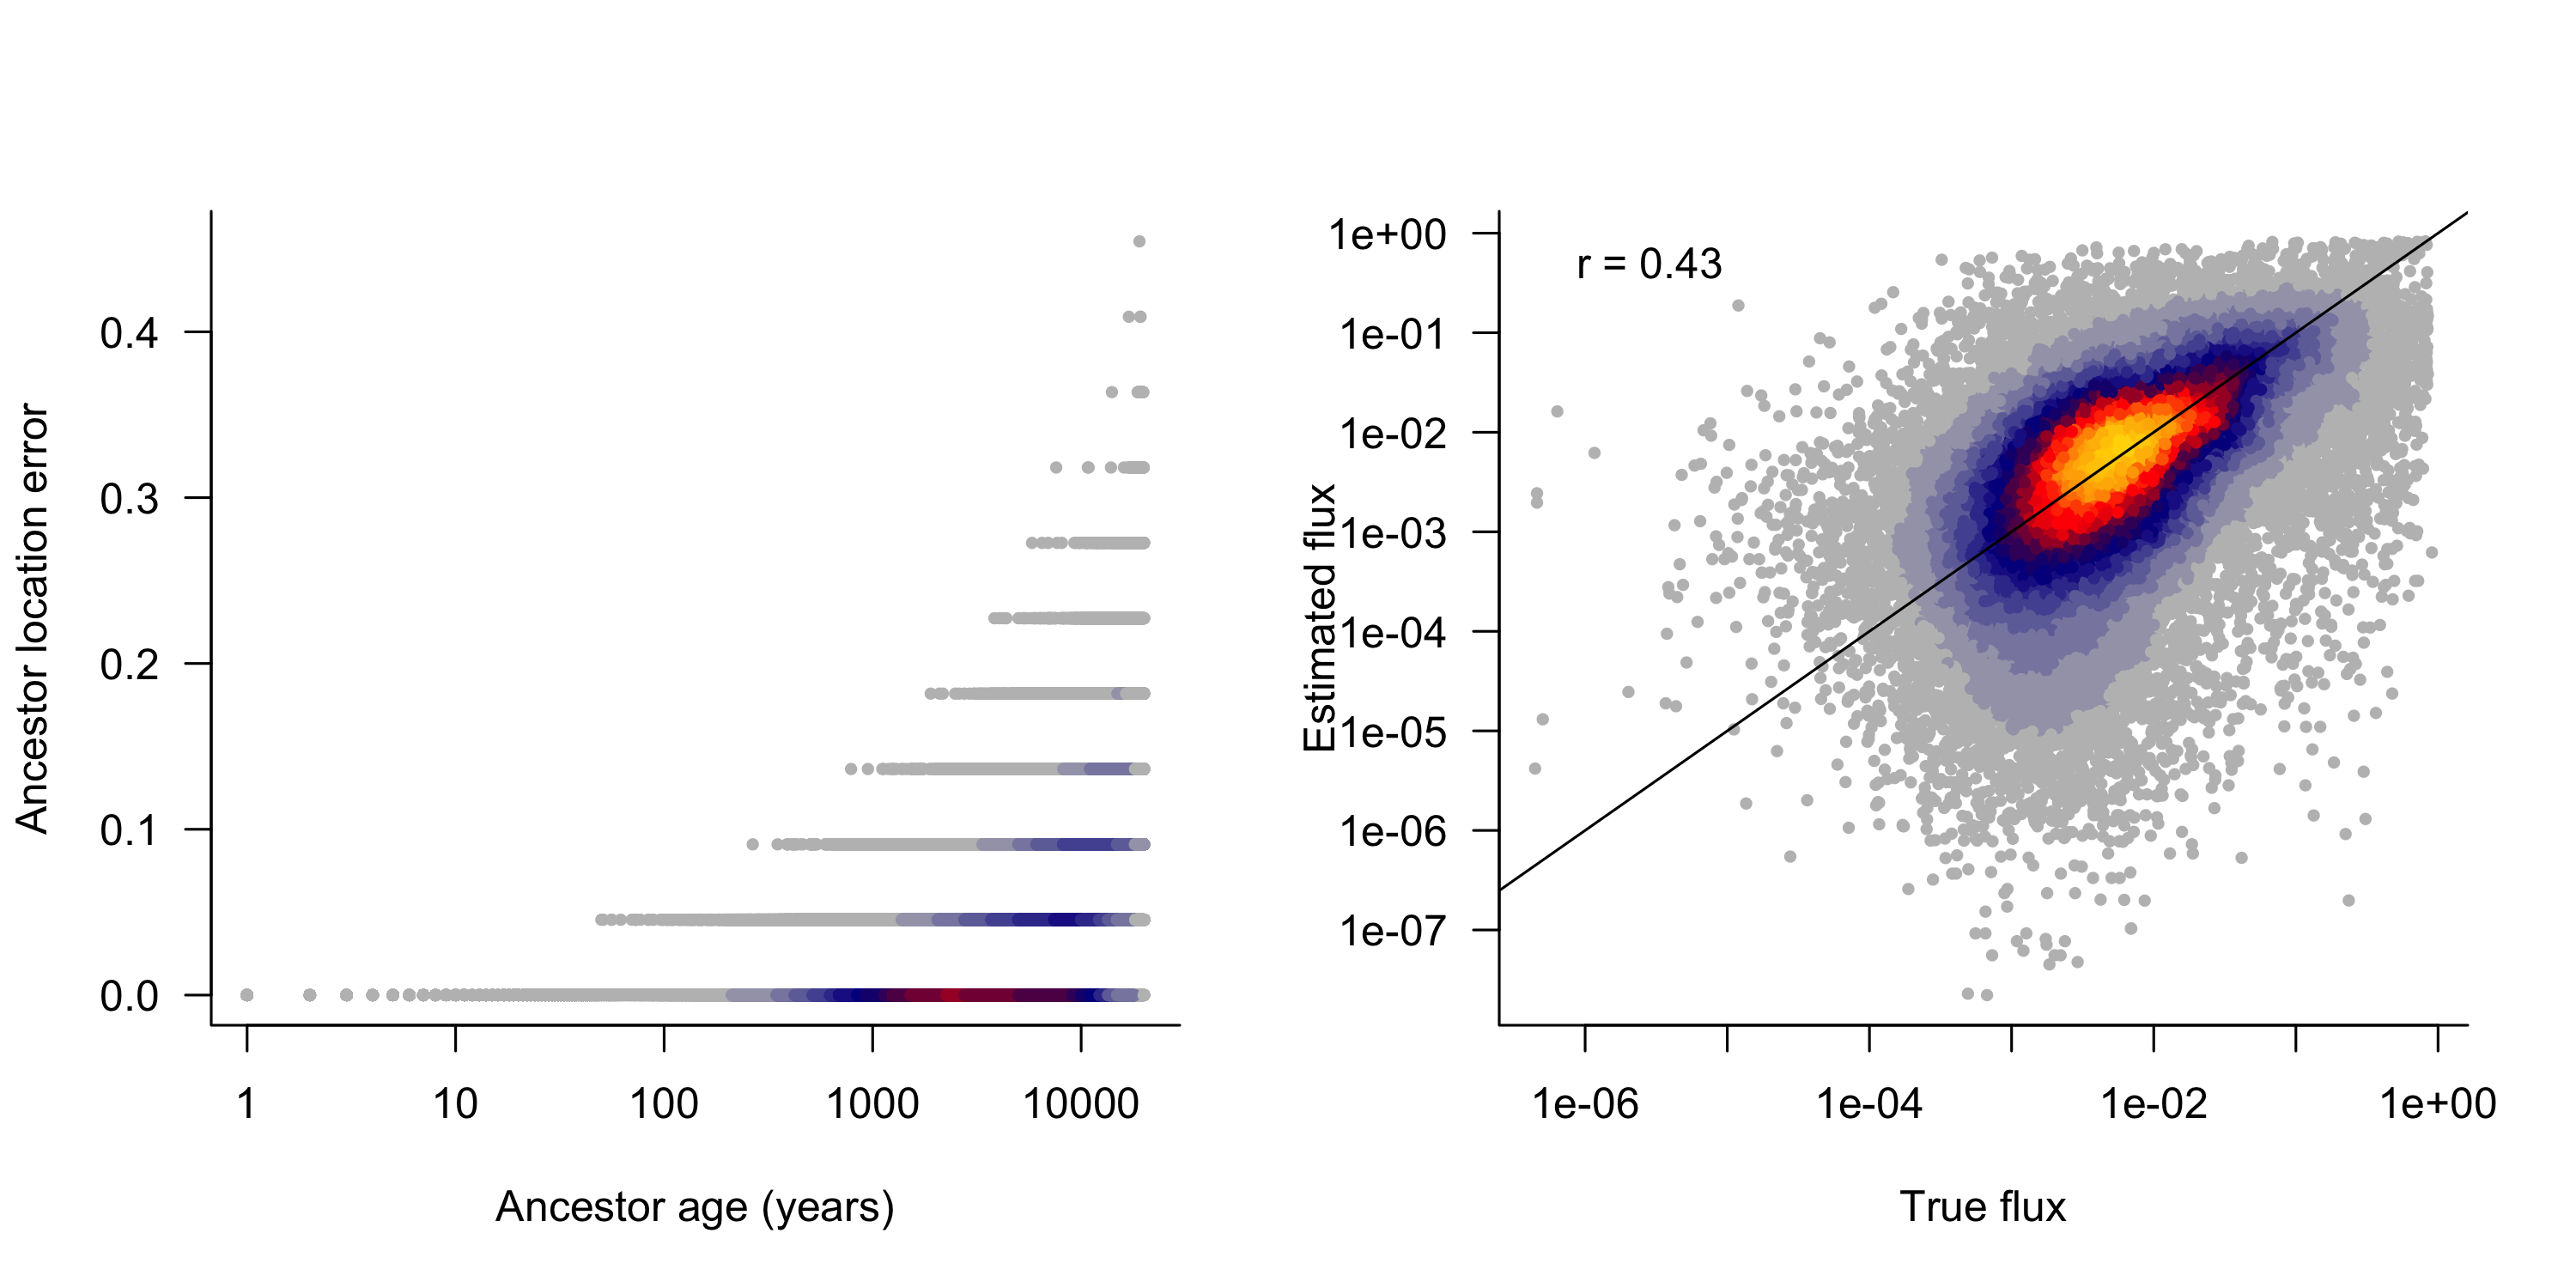
\includegraphics[width=\textwidth]{figs/ooa-sim-flux-cor}
\caption{Ancestor location error (left) and correlation between estimated 
ancestry flux and true ancestry flux (right) across all out of Africa 
simulations. Ancestor location error is measured as the graph distance between
true and estimated locations expressed as a proportion of the maximum graph distance
between any two geographic states. True ancestry flux is computed by using the true ancestor
locations (for both coalescent and unary tree sequence nodes) in the computation
of the flux coefficient described in the main text. Here we use a single 
window corresponding to the entire temporal span of the recorded tree sequences
(20,000 years). Estimates of ancestry flux, while broadly correlated with true 
flux, tend to be much noisier than ancestor location estimates, reflecting both 
the error in ancestor location estimates and the error incurred by interpolating 
migration routes between estimated locations of coalescent nodes.
}
\label{fig:ooa-flux-cor}
\end{figure}

\begin{figure}
\centering
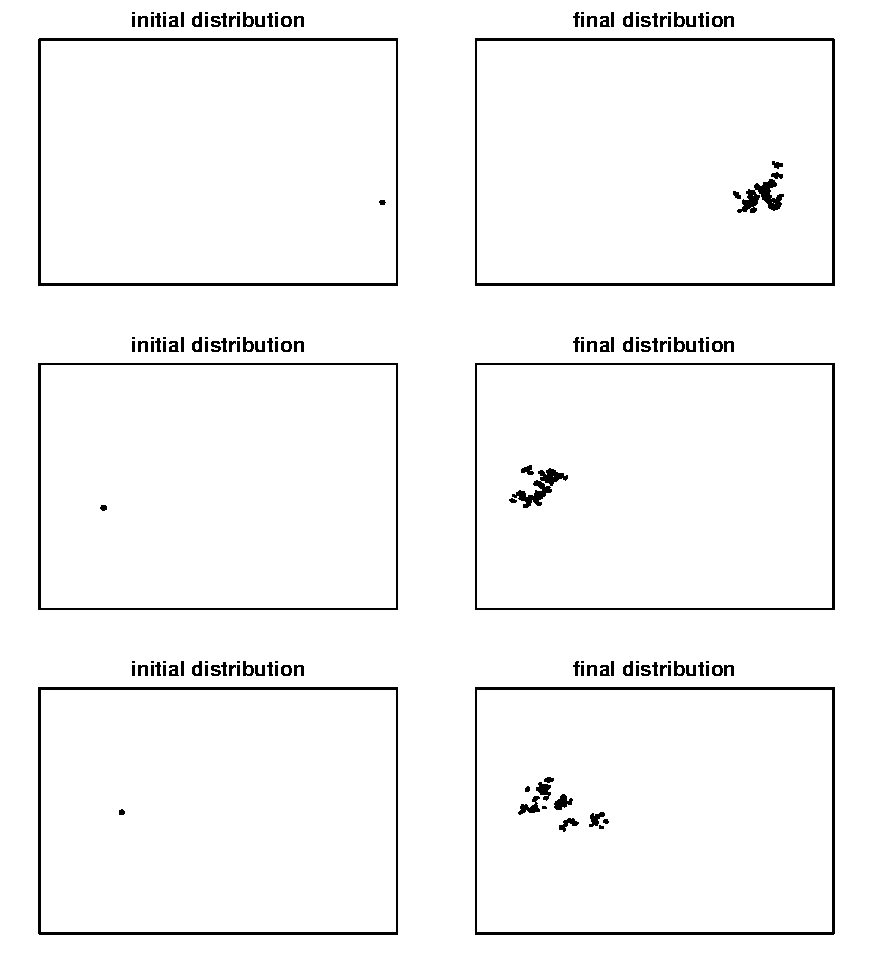
\includegraphics[width=\textwidth]{figs/homog-init}
\caption{Three randomly chosen examples of the initial and final distribution
of individuals in SLiM simulations on a landscape with uniform carrying capacity. In all cases the
landscape is a square with reflecting boundaries and side lengths of 1000$S$, 
where $S$ is the standard deviation of individual dispersal kernels. All
simulations were seeded from a founding population of 30 individuals and were
terminated after 10,000 generations.
}
\label{fig:homog-init}
\end{figure}


\begin{figure}
\centering
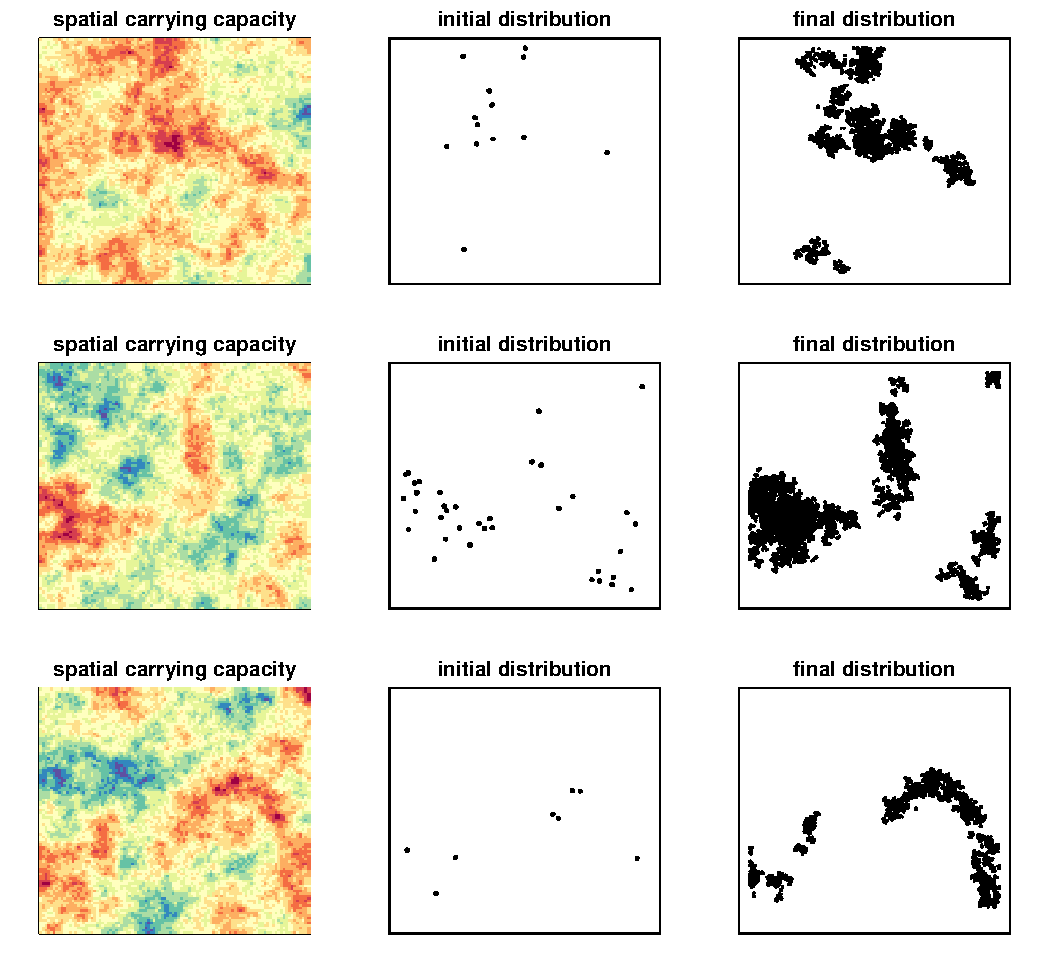
\includegraphics[width=\textwidth]{figs/hetero-init}
\caption{Three randomly chosen examples of the initial and final distribution
of individuals in SLiM simulations on a landscape with spatially variable
carrying capacity. In all cases the landscape is a square with reflecting 
boundaries and side lengths of 1000$S$, where $S$ is the standard deviation of 
individual dispersal kernels. All simulations were seeded from 30 individuals
at each of 300 locations scattered uniformly at random across the landscape and 
were terminated after 10,000 generations.
}
\label{fig:hetero-init}
\end{figure}

\end{linenumbers}

\end{document}
